\documentclass[12pt,a4paper]{article}
% Compiler: pdfLaTeX (Overleaf default)
\usepackage[T2A,T1]{fontenc}
\usepackage[utf8]{inputenc}
\usepackage[russian,english]{babel}
\usepackage[a4paper,left=3cm,right=1.5cm,top=2cm,bottom=2cm]{geometry}
\usepackage[expansion=false]{microtype}
\usepackage{setspace}
\onehalfspacing
\usepackage{amssymb}
\usepackage{pifont}
\usepackage{wasysym}
\usepackage{array}
\usepackage{tabularx}
\usepackage{xltabular}
\usepackage{booktabs}
\usepackage[table]{xcolor}
\usepackage{caption}
\captionsetup{font=small,labelfont=bf,justification=raggedright,singlelinecheck=false}
\captionsetup[table]{position=top,skip=4pt}
\usepackage{enumitem}
\setlist{nosep,leftmargin=1.6em}
\usepackage[nobottomtitles*]{titlesec}
\renewcommand{\bottomtitlespace}{0.15\textheight}
\titleformat{\section}{\large\bfseries}{\thesection.}{0.6em}{}
\titleformat{\subsection}{\normalsize\bfseries}{\thesubsection.}{0.6em}{}
\titlespacing*{\section}{0pt}{1.2em}{0.5em}
\titlespacing*{\subsection}{0pt}{0.9em}{0.4em}
\usepackage{needspace}
\usepackage{etoolbox}
\usepackage{fancyhdr}
\pagestyle{fancy}\fancyhf{}
\fancyfoot[C]{\thepage}
\renewcommand{\headrulewidth}{0pt}
\usepackage{xurl}
\usepackage[colorlinks=true,linkcolor=black,citecolor=blue!50!black,urlcolor=blue!50!black]{hyperref}
\setlength{\parindent}{1.25cm}
\setlength{\parskip}{0pt}
\setlength{\emergencystretch}{3em}
\urlstyle{same}

% table style
\definecolor{headgray}{gray}{0.90}
\definecolor{linegray}{gray}{0.70}
\newcolumntype{L}{>{\raggedright\arraybackslash}X}
\newcolumntype{P}[1]{>{\raggedright\arraybackslash}p{#1}}
\newcolumntype{C}[1]{>{\centering\arraybackslash}p{#1}}
\newcommand{\rl}{\arrayrulecolor{linegray}\hline\arrayrulecolor{black}}
\newcommand{\thead}{\rowcolor{headgray}}

% comparison marks
\newcommand{\yes}{\ensuremath{\checkmark}}
\newcommand{\no}{\ding{55}}
\newcommand{\partly}{\LEFTcircle}
\newcommand{\ru}[1]{\foreignlanguage{russian}{#1}}
\newcommand{\doi}[1]{doi: \href{https://doi.org/#1}{#1}}

% title page
\newcommand{\maketitlepage}[1]{%
\begin{titlepage}
\centering
{\large Astana IT University\par}
{\normalsize School of Software Engineering\par}
\vspace{4.5cm}
{\normalsize Diploma Project\par}
\vspace{0.6cm}
{\Large\bfseries Development of a System for Detecting and Anonymizing Personal Data Before Sending Text to Artificial Intelligence Services\par}
\vspace{1.2cm}
{\LARGE #1\par}
\vfill
\begin{flushright}
\begin{tabular}{@{}l@{}}
\textbf{Authors:} Dossan Amina, Abzhamal Nazerke\\
\textbf{Educational programme:} Software Engineering\\
\textbf{Supervisor:} Sakhipov A.A., PhD,\\ \hspace{2.2cm}Assistant Professor
\end{tabular}
\end{flushright}
\vspace{2.5cm}
{\normalsize Astana, 2026\par}
\end{titlepage}
\setcounter{page}{2}}
\usepackage{graphicx}
\usepackage{float}
\graphicspath{{screens/}}
\begin{document}
\maketitlepage{User Interface Prototype}

\tableofcontents
\newpage

\section{Introduction}

This document presents the user interface (UX) prototype of the PII Anonymization Gateway. The prototype shows how users interact with the browser extension when sending text to ChatGPT or Gemini, how administrators configure the system, and how internal systems use the programming interface. Its purpose is to validate the requirements defined in the document \emph{Requirements Specification} before implementation and to serve as the basis for user testing.

\section{Prototype Description}

The prototype is a high-fidelity static prototype consisting of 18 screens. The main user scenario (screens U1--U4) is clickable and can be walked through in order. The interface of the user screens is in Russian, screen U6 shows the Kazakh interface, and the extension supports Kazakh, Russian and English (FR-5.7). All names, identifiers, phone numbers and addresses on the screens are fictitious; IIN, BIN, IBAN and card numbers are generated in a valid format.

The screens are grouped as follows:
\begin{itemize}
\item \emph{User scenario in the browser extension} (U1--U8): entering text, reviewing detected data, preview of the anonymized text, restored response, blocking by policy, Kazakh and mixed-language text, and failure of the anonymization server;
\item \emph{Extension window} (X1, X2): sign-in and status;
\item \emph{Administration panel} (A1--A6): sign-in, statistics, policies, log, users and roles, security settings;
\item \emph{Programming interface} (P1): examples of API requests and responses.
\end{itemize}

The exported screens are stored in the \texttt{docs/ux-prototype/screens} directory of the repository.

\section{Design Decisions Based on the User Survey}

The prototype reflects the results of the user survey ($n=35$) described in the document \emph{Evidence of Relevance} (Table~\ref{tab:decisions}).

\begin{table}[H]
\caption{Survey findings and design decisions}\label{tab:decisions}
\small
\begin{tabularx}{\linewidth}{P{5.6cm}LP{1.6cm}}
\toprule
\thead \textbf{Finding} & \textbf{Design decision} & \textbf{Screens} \\ \midrule
57\% want to review detected data before sending; 14\% prefer automatic replacement & Review before sending is the default mode; the automatic mode can be enabled in the extension window if the administrator allows it & U2, X1 \\ \rl
51\% prefer detecting all personal data even with occasional false alarms & Low-confidence detections are shown as unmarked suggestions; the user can mark missed data manually & U2, U7 \\ \rl
71\% use several languages or mix them; 77\% use Kazakh or mixed prompts & Detected languages are shown; the extension interface is available in Kazakh & U6, U7 \\ \rl
89\% accept an additional delay of at least 1--3 s & Processing time is shown to the user and to the administrator & U3, A2 \\ \rl
Concerns about confidentiality and trust in the tool & The user sees exactly what the AI service receives; the log contains no original values; text is not sent if it could not be checked & U3, A4, U8 \\ \rl
54\% want a detection log and per-type rules & Policies per data type and a filterable log & A3, A4 \\
\bottomrule
\end{tabularx}
\end{table}

\section{Main User Scenario}

The main scenario corresponds to use cases UC-1 and UC-2. The user writes a request in ChatGPT that contains the name, IIN, identity document number and IBAN of a client, the BIN of an organization, an address and the contacts of a manager.

\begin{figure}[H]
\centering
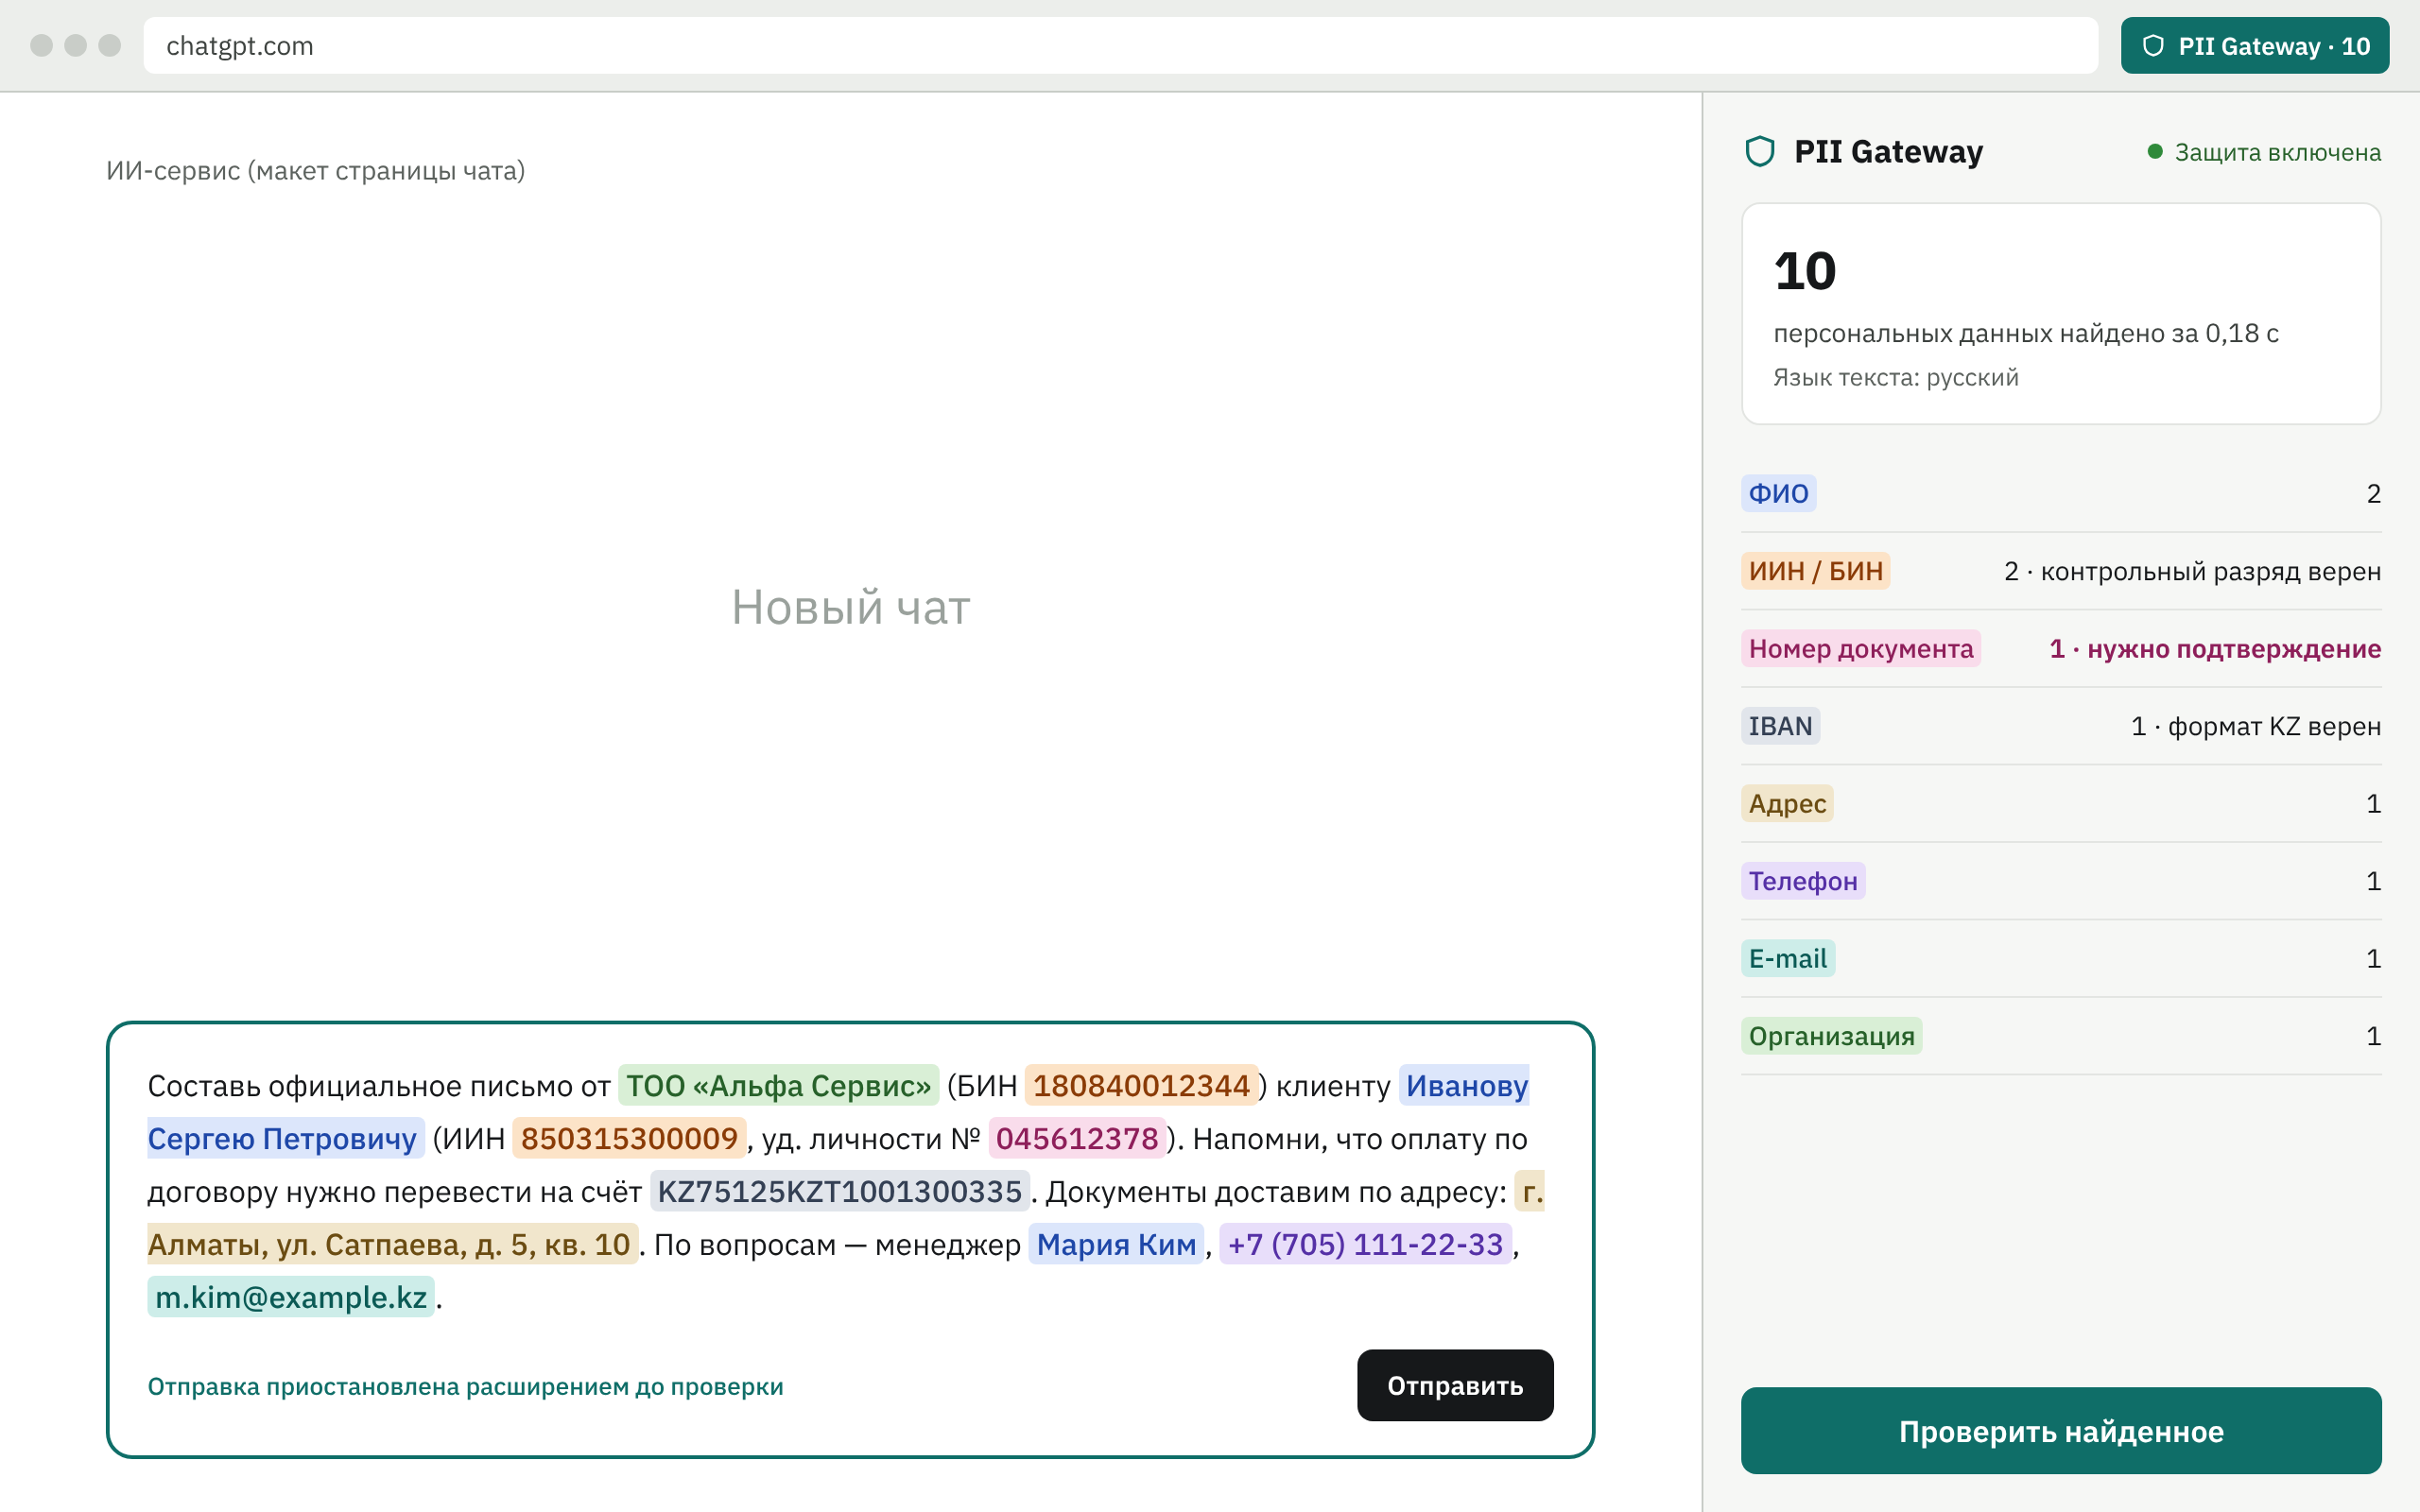
\includegraphics[width=\linewidth]{01-U1-Compose.png}
\caption{U1. Text input: detected personal data are highlighted by type directly in the input field; IIN and BIN are marked as validated by the check digit}\label{fig:u1}
\end{figure}

\begin{figure}[H]
\centering
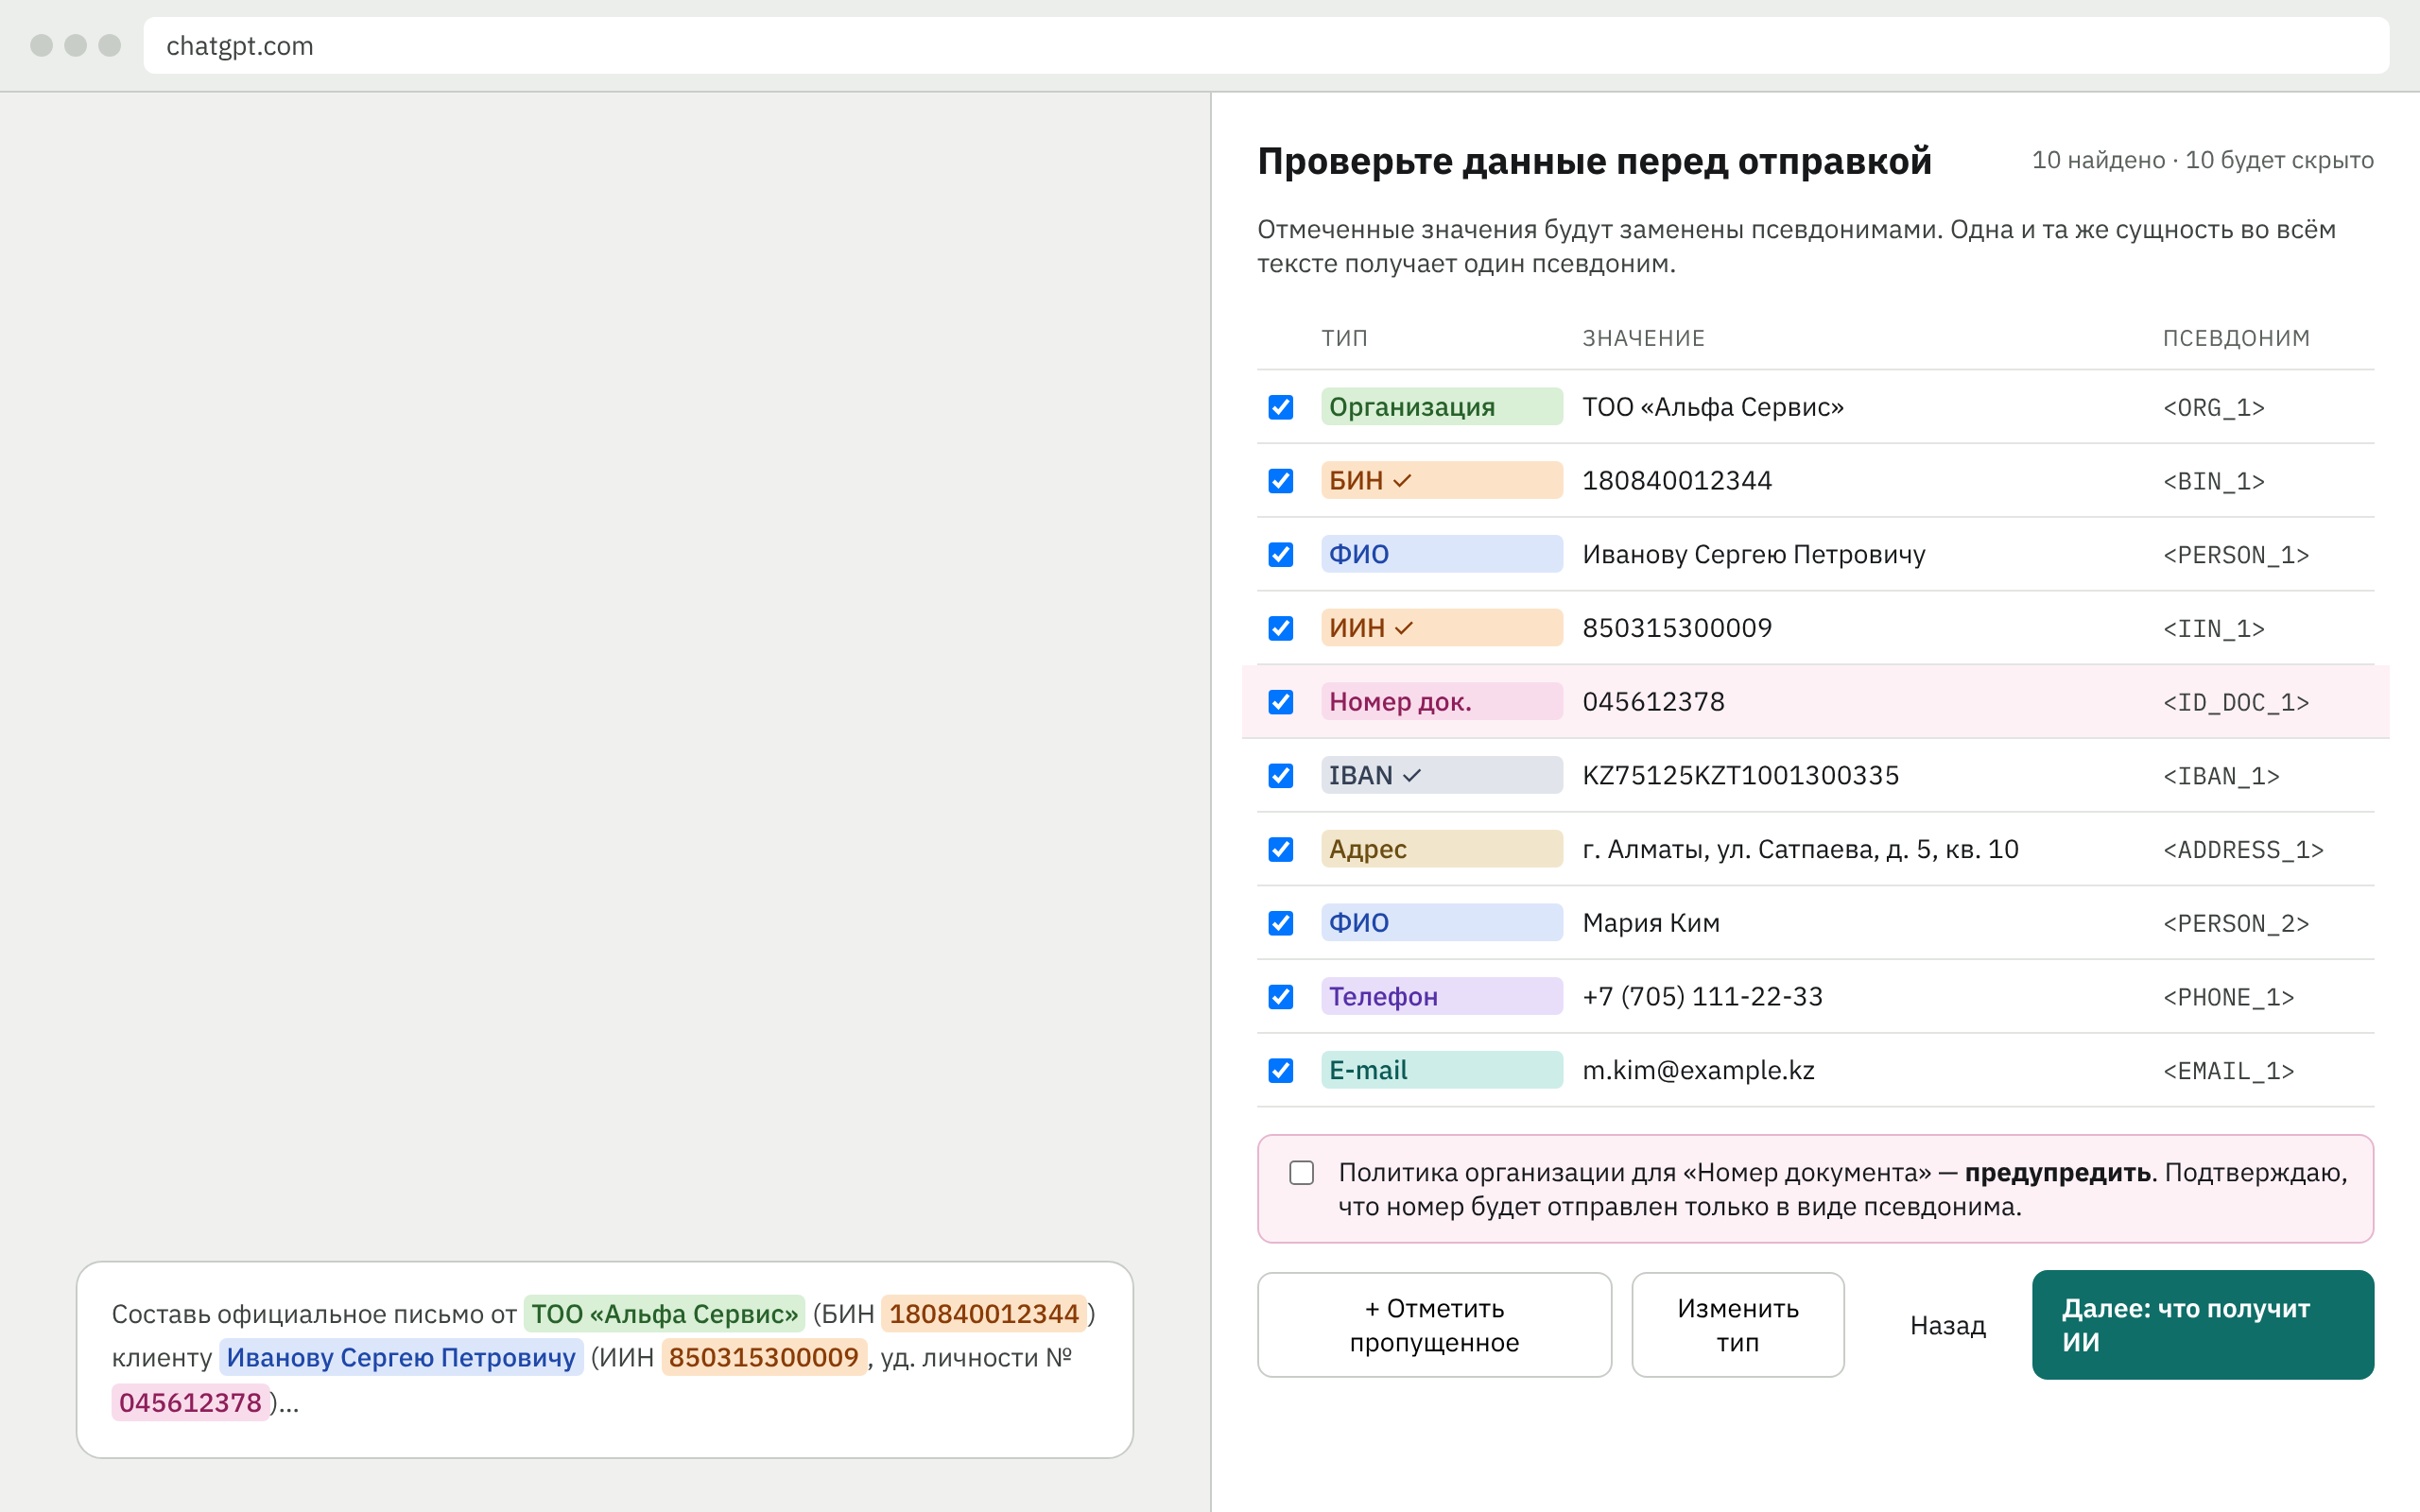
\includegraphics[width=\linewidth]{02-U2-Review.png}
\caption{U2. Review of detected data: the user can unmark a value, change its type or mark missed data; the policy ``warn'' for the identity document number requires explicit confirmation}\label{fig:u2}
\end{figure}

\begin{figure}[H]
\centering
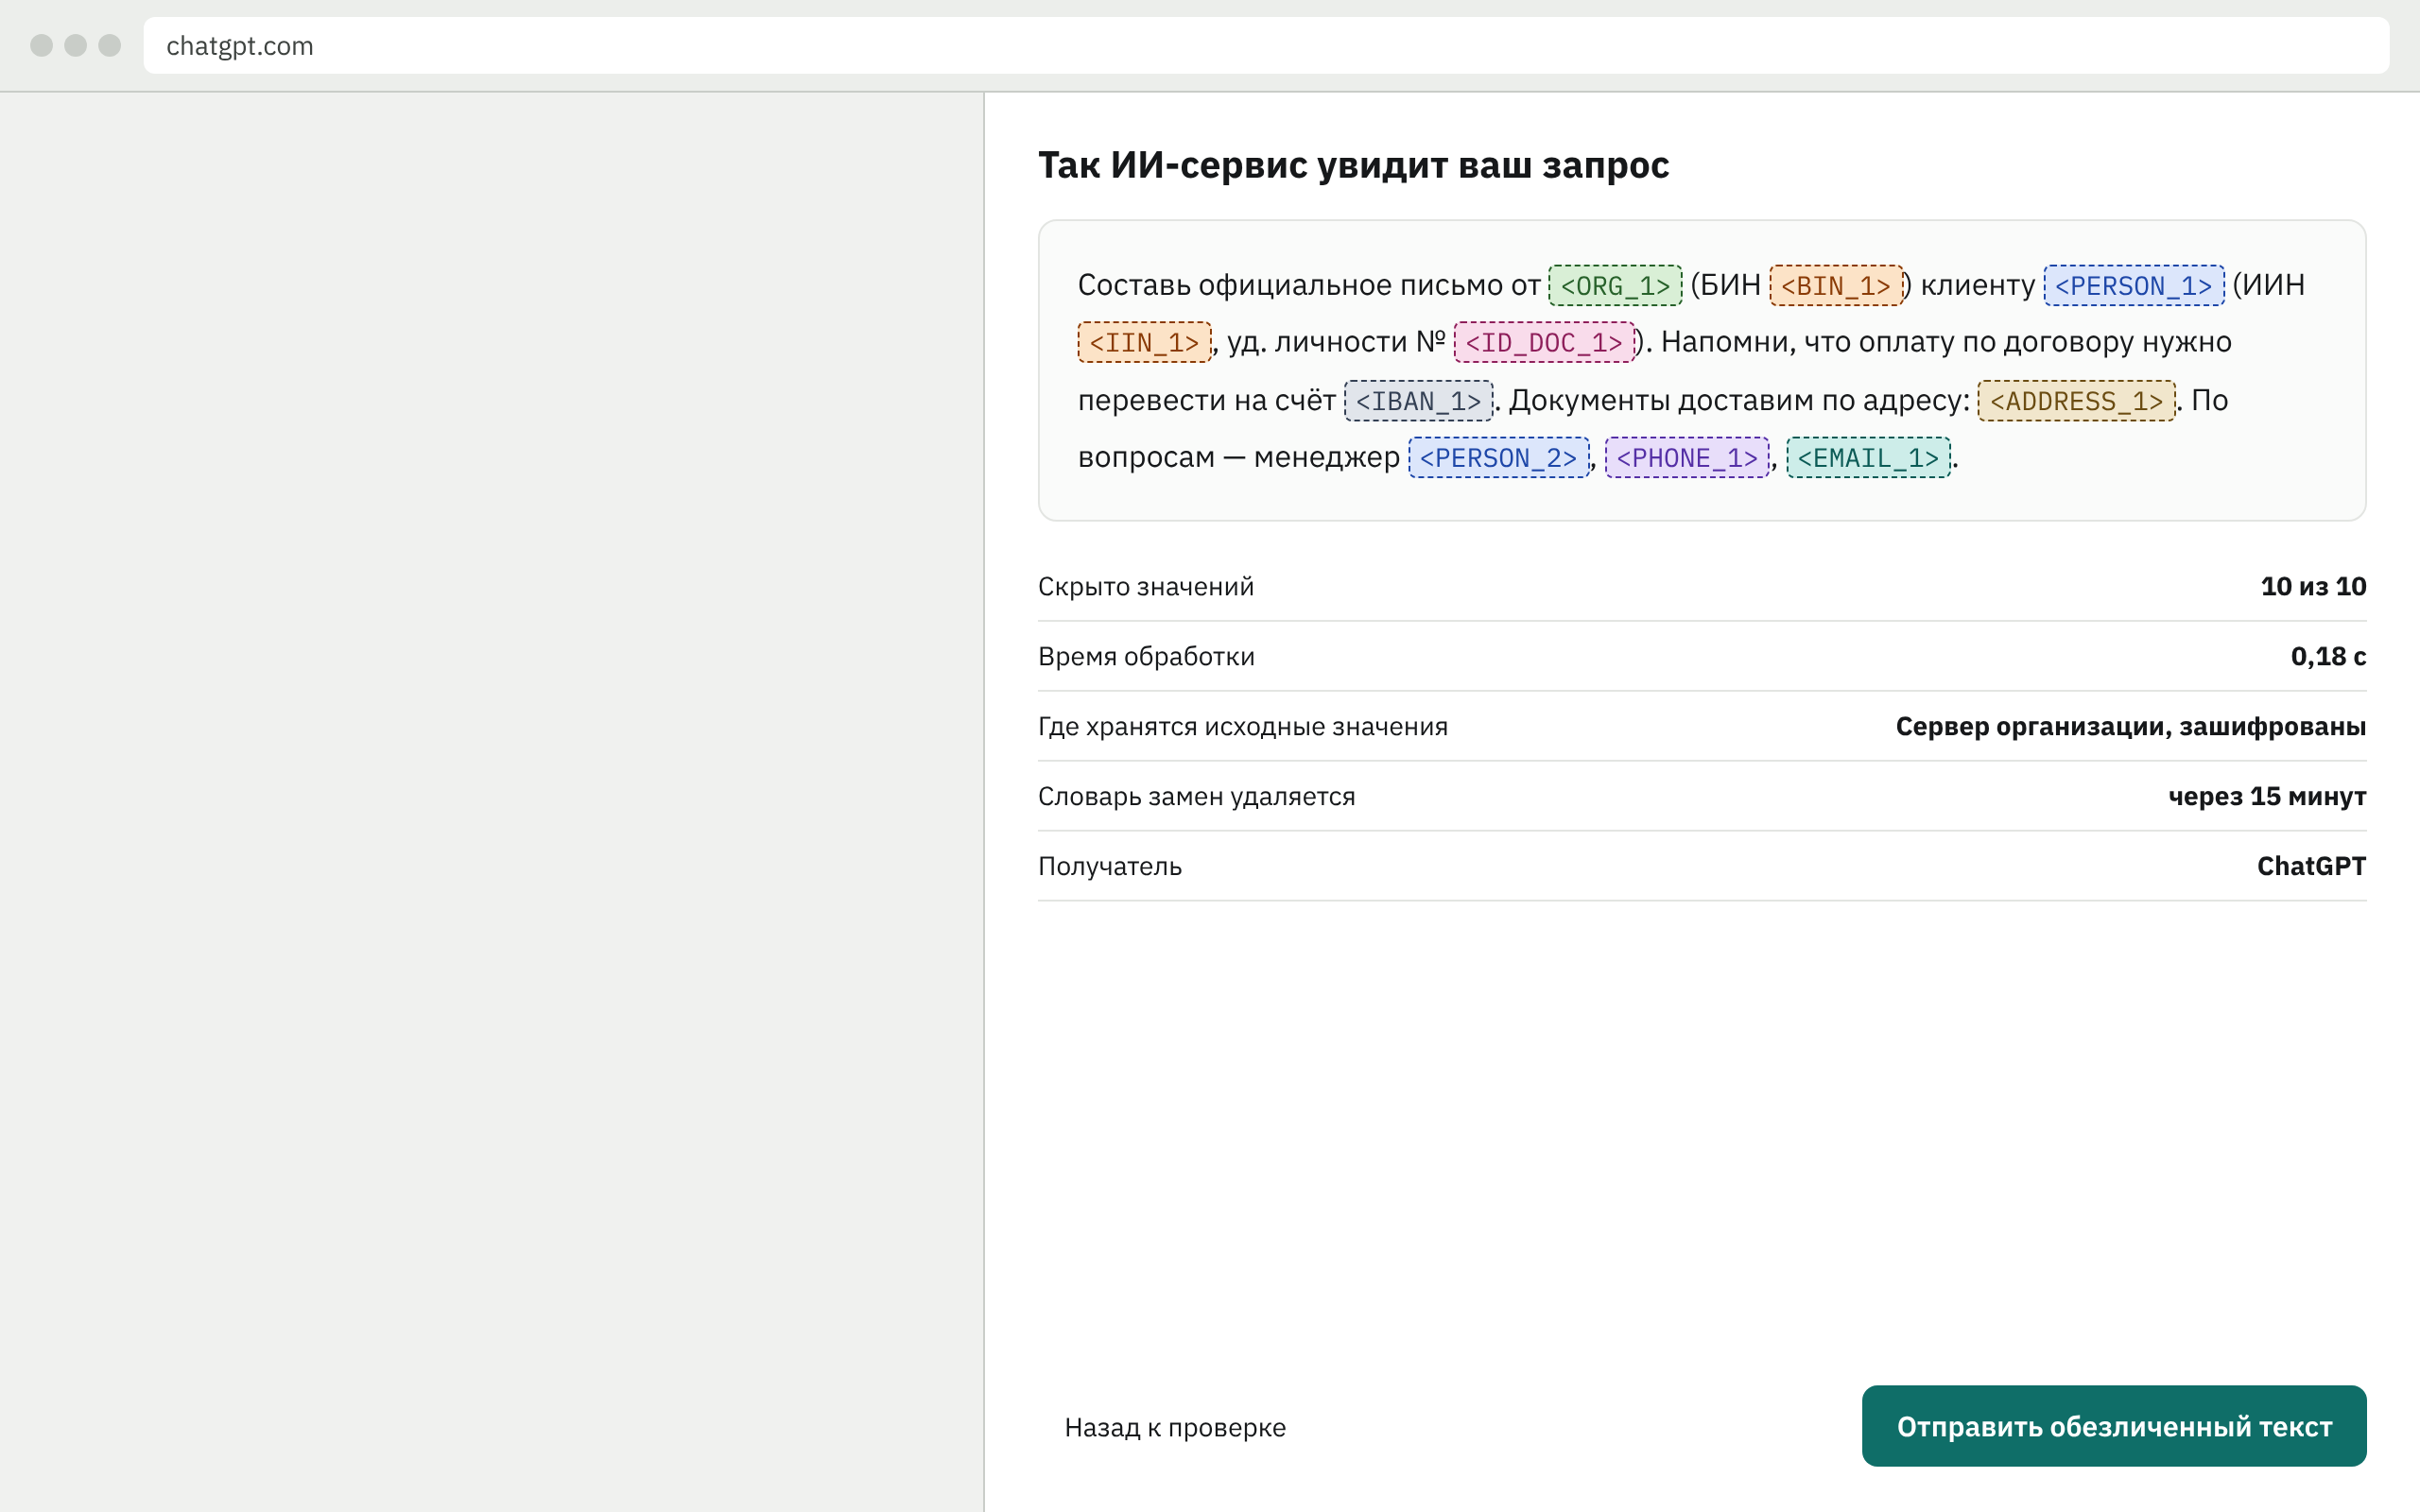
\includegraphics[width=\linewidth]{03-U3-Preview.png}
\caption{U3. Preview of the text that the AI service will receive and the processing time}\label{fig:u3}
\end{figure}

\begin{figure}[H]
\centering
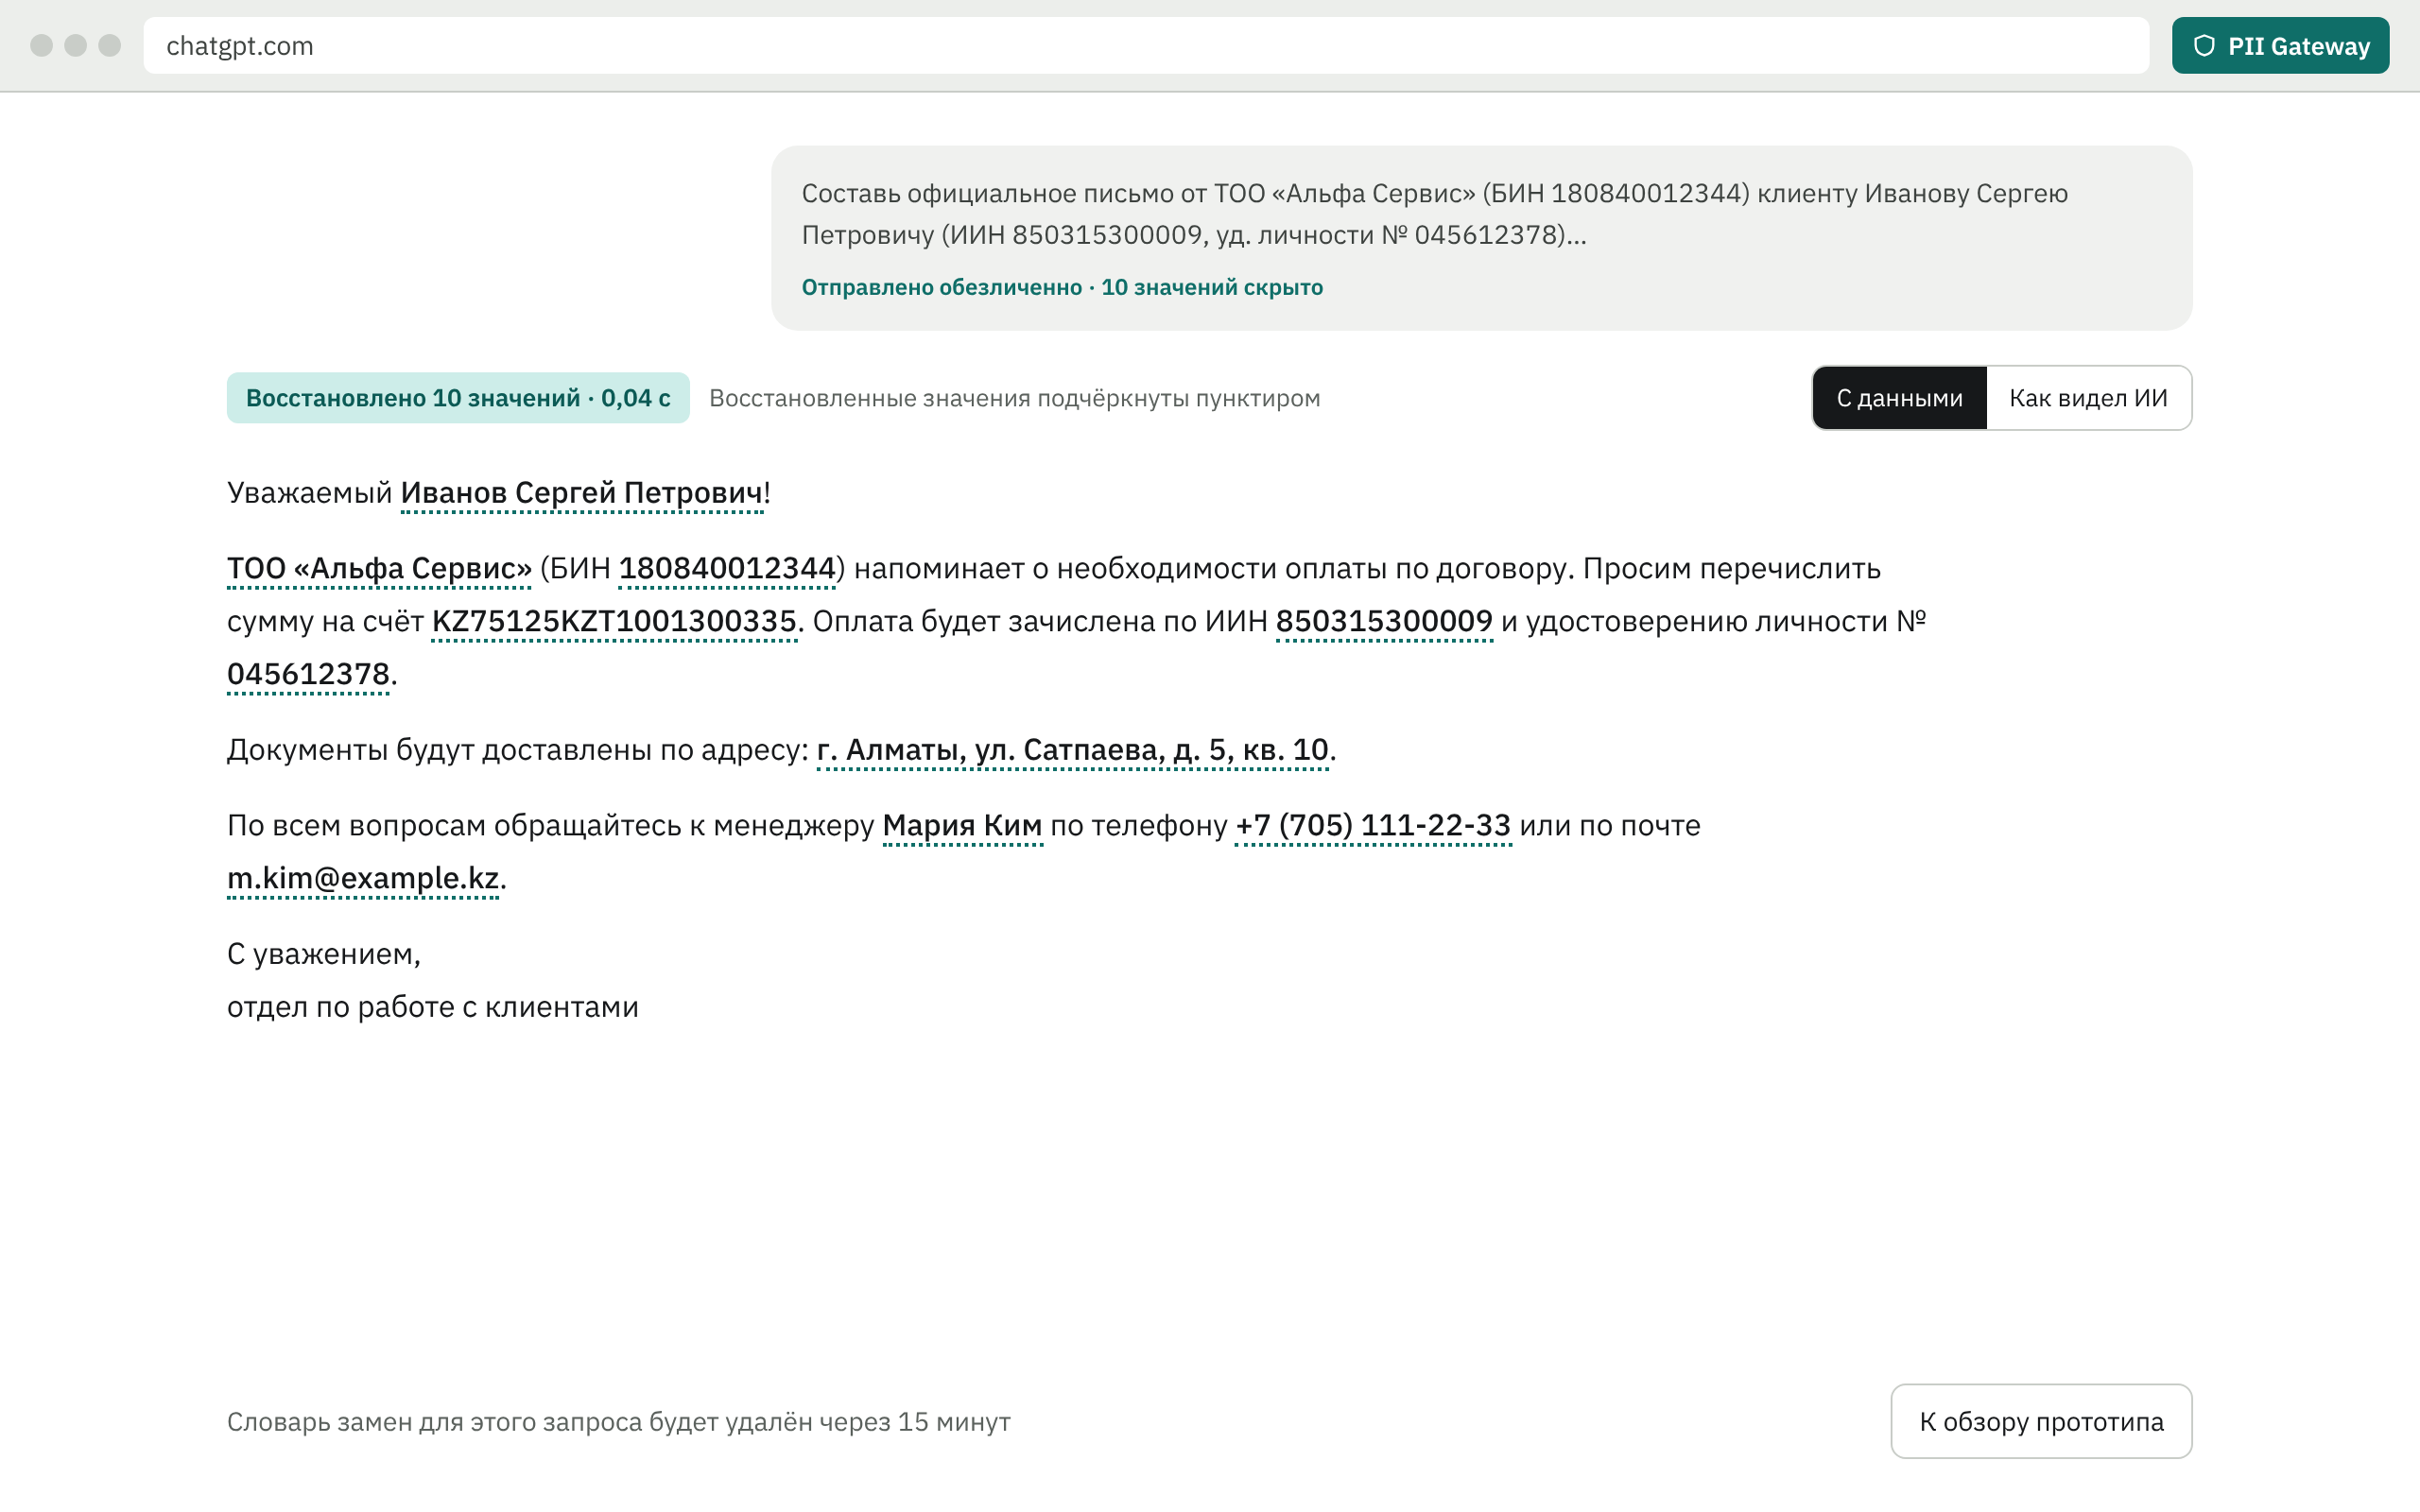
\includegraphics[width=\linewidth]{04-U4-Response.png}
\caption{U4. Response with restored values: restored values are underlined, and the user can switch to the view ``as the AI saw it''}\label{fig:u4}
\end{figure}

\section{Alternative Scenarios}

\begin{figure}[H]
\centering
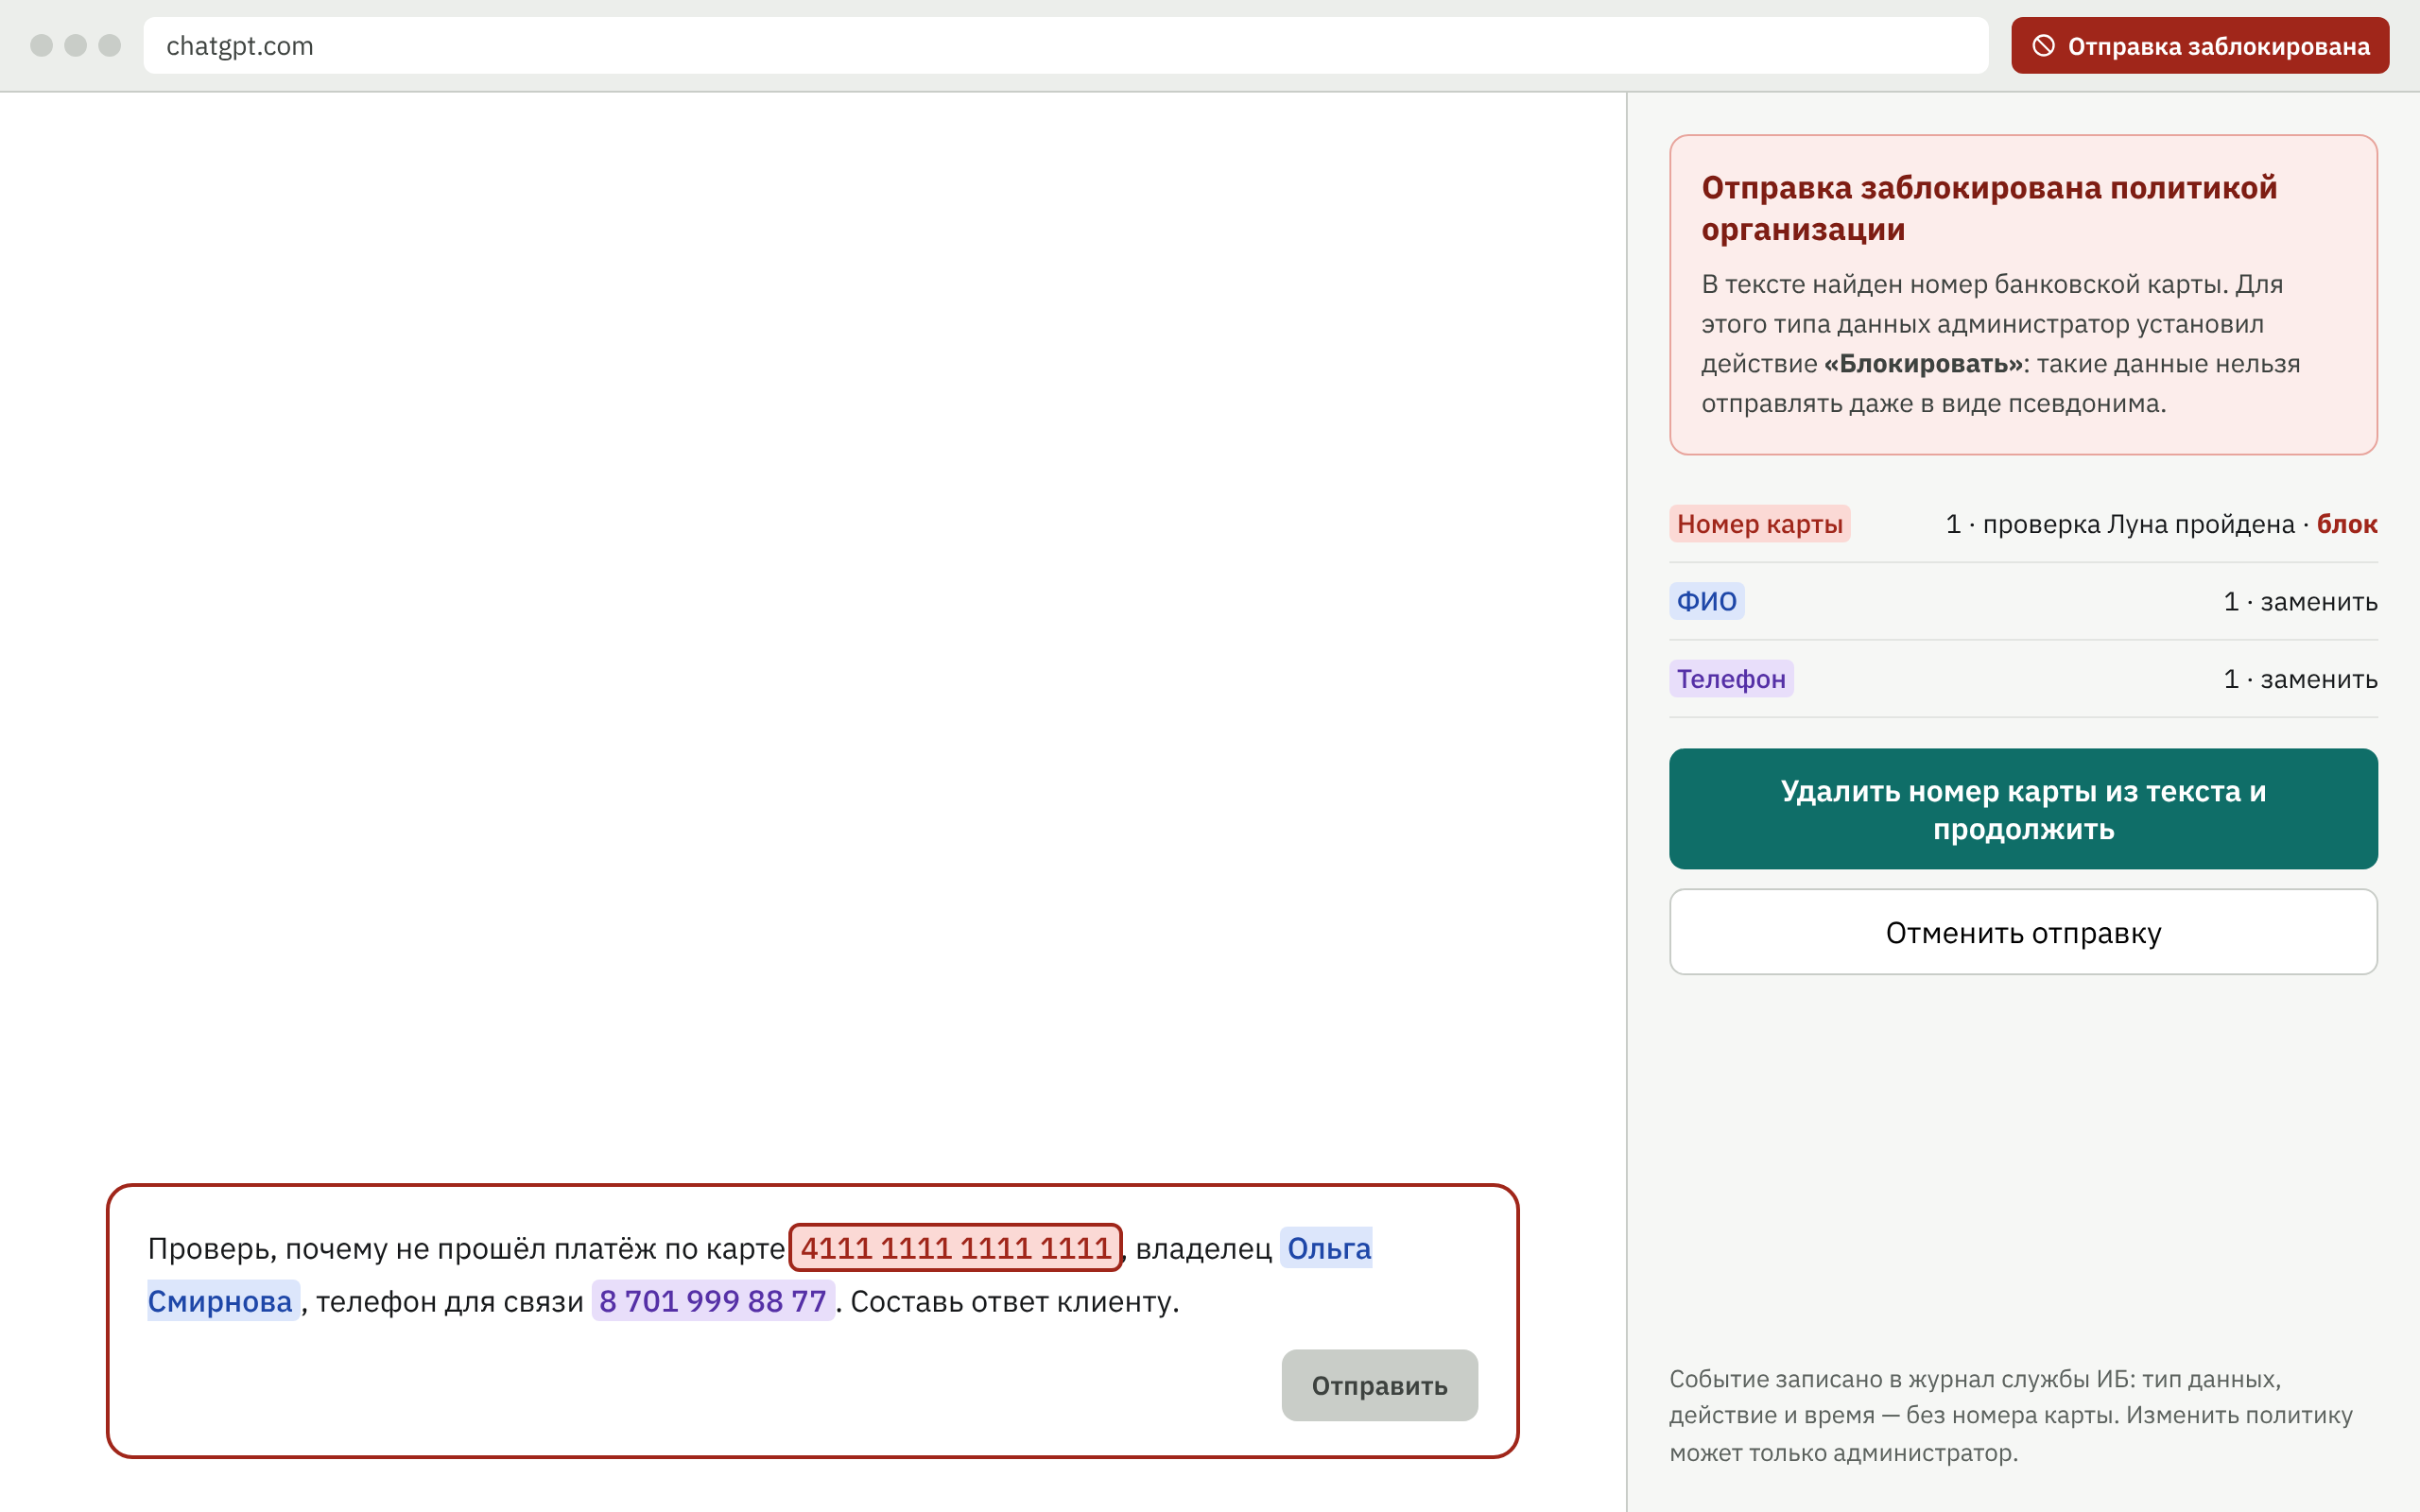
\includegraphics[width=\linewidth]{05-U5-Blocked.png}
\caption{U5. Blocking by policy: the text contains a bank card number validated by the Luhn algorithm, for which the administrator set the action ``block'' (UC-3)}\label{fig:u5}
\end{figure}

\begin{figure}[H]
\centering
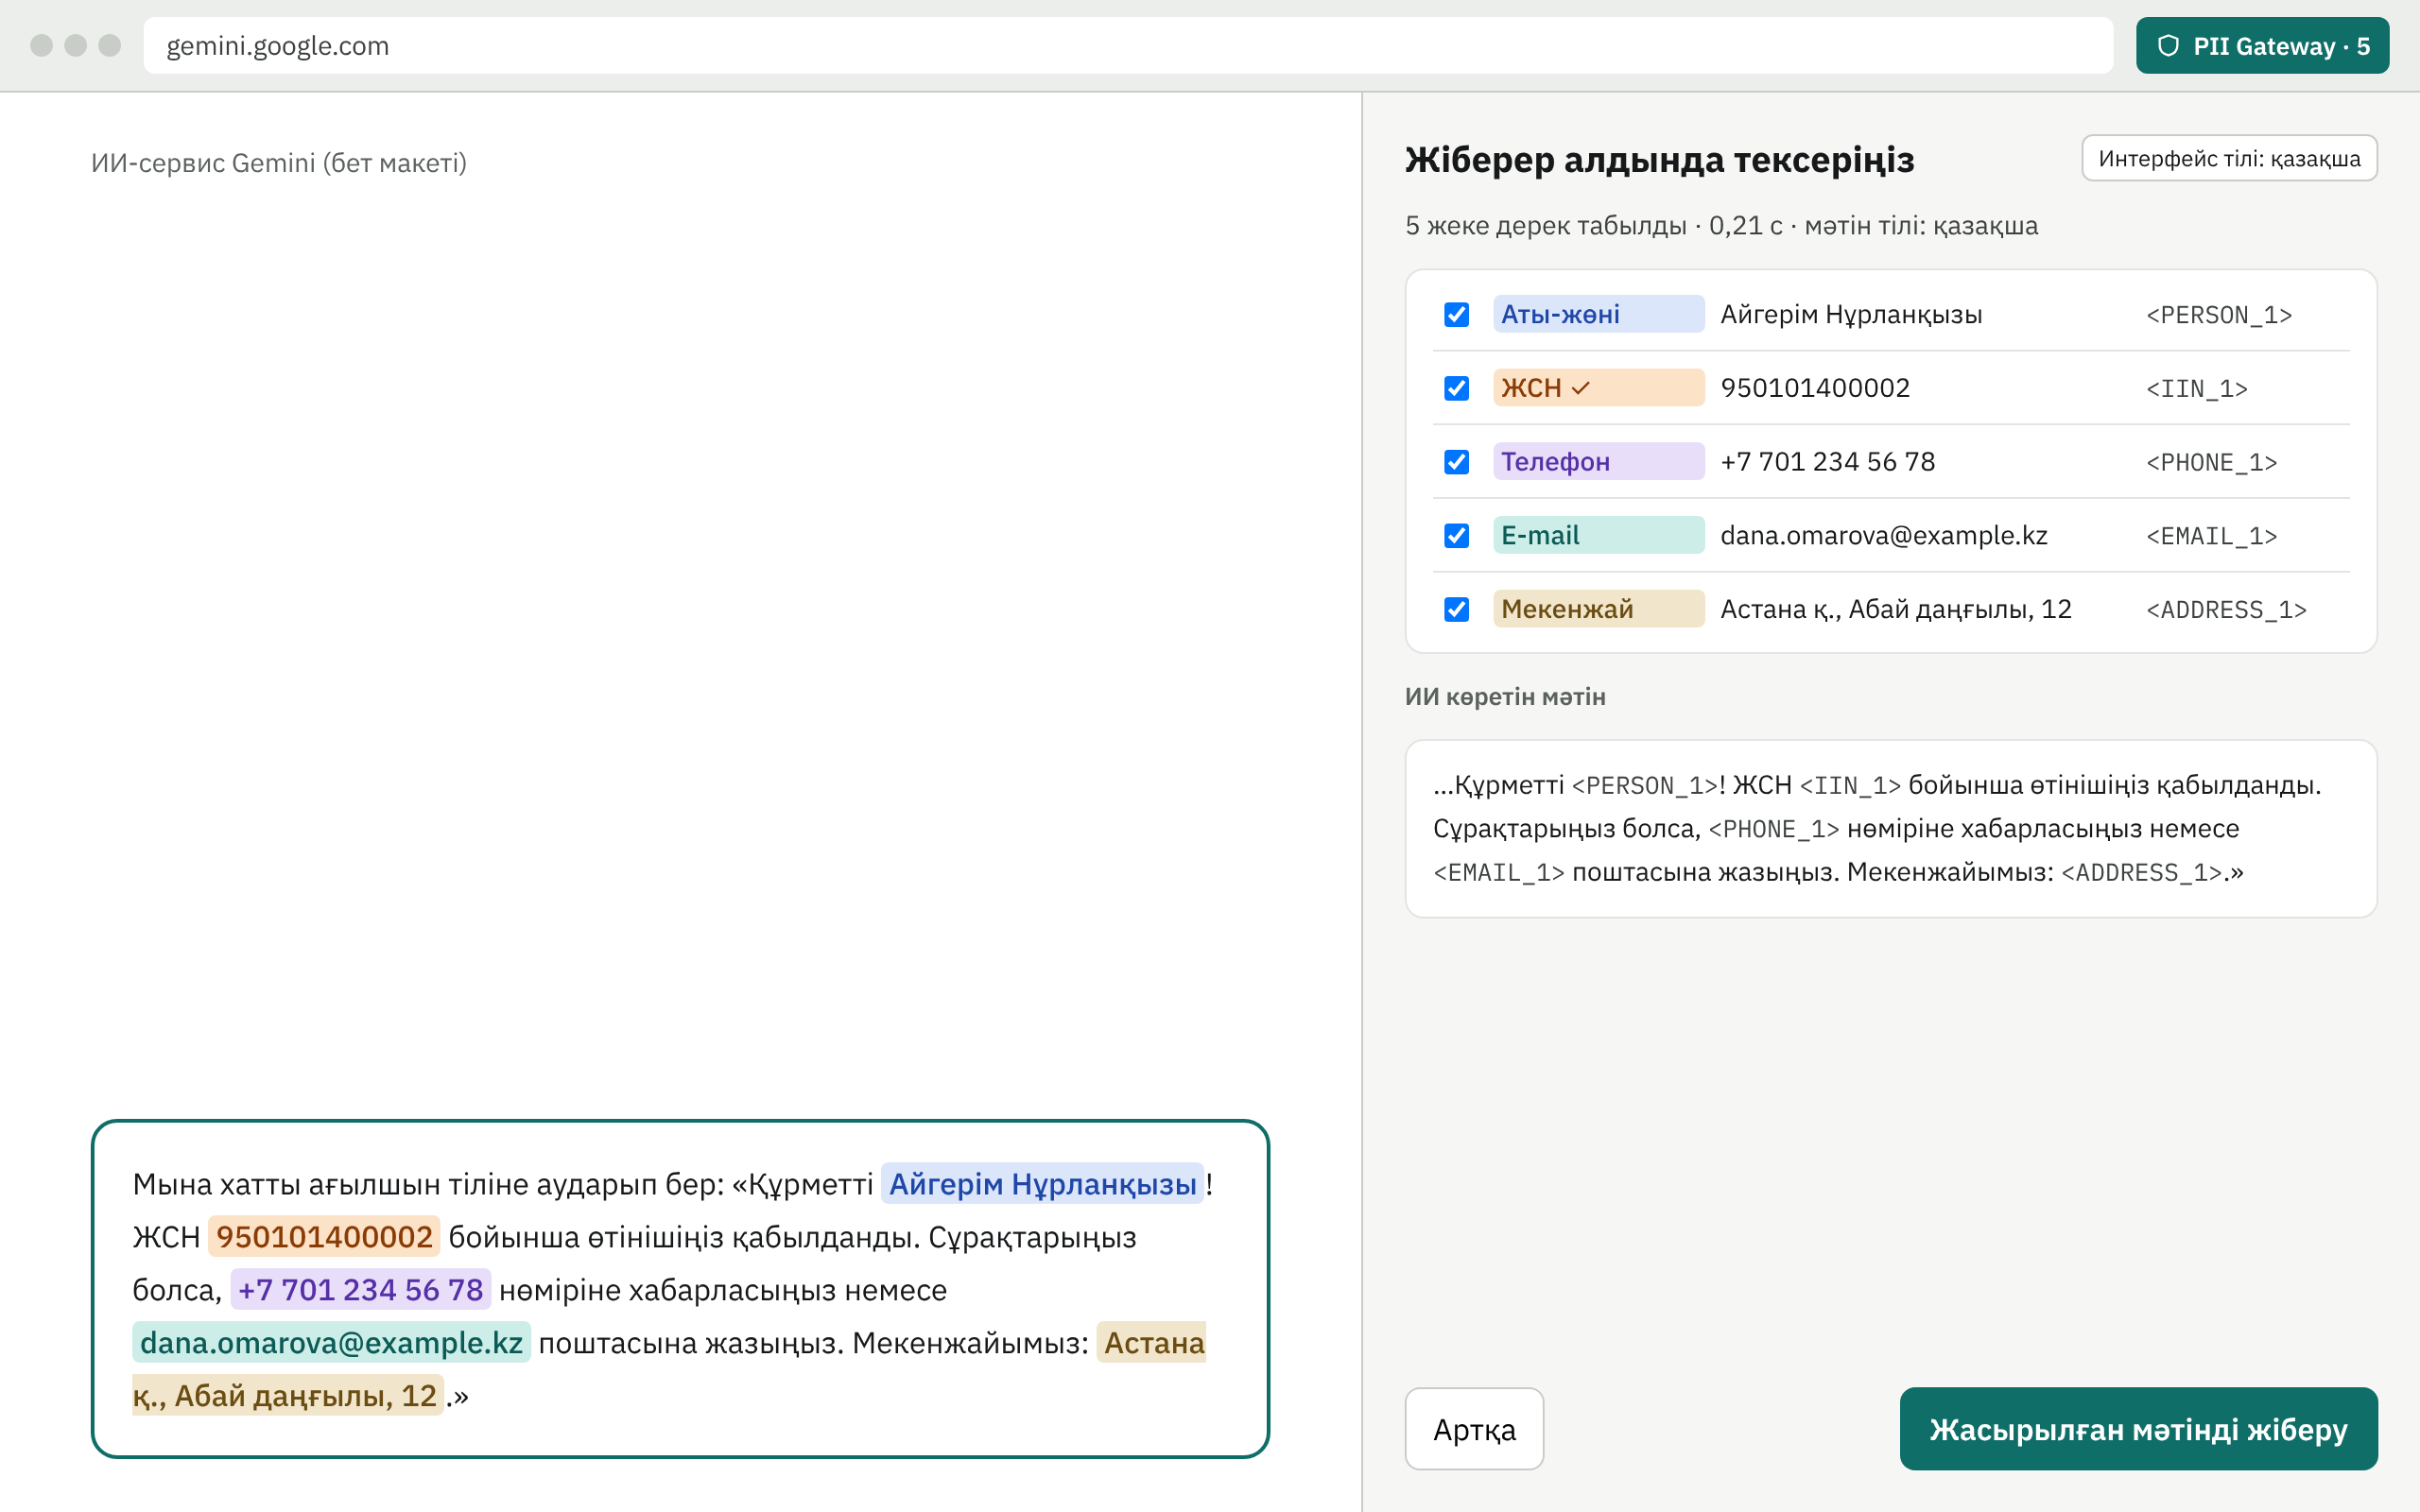
\includegraphics[width=\linewidth]{06-U6-Kazakh.png}
\caption{U6. Gemini with a Kazakh text and the Kazakh extension interface}\label{fig:u6}
\end{figure}

\begin{figure}[H]
\centering
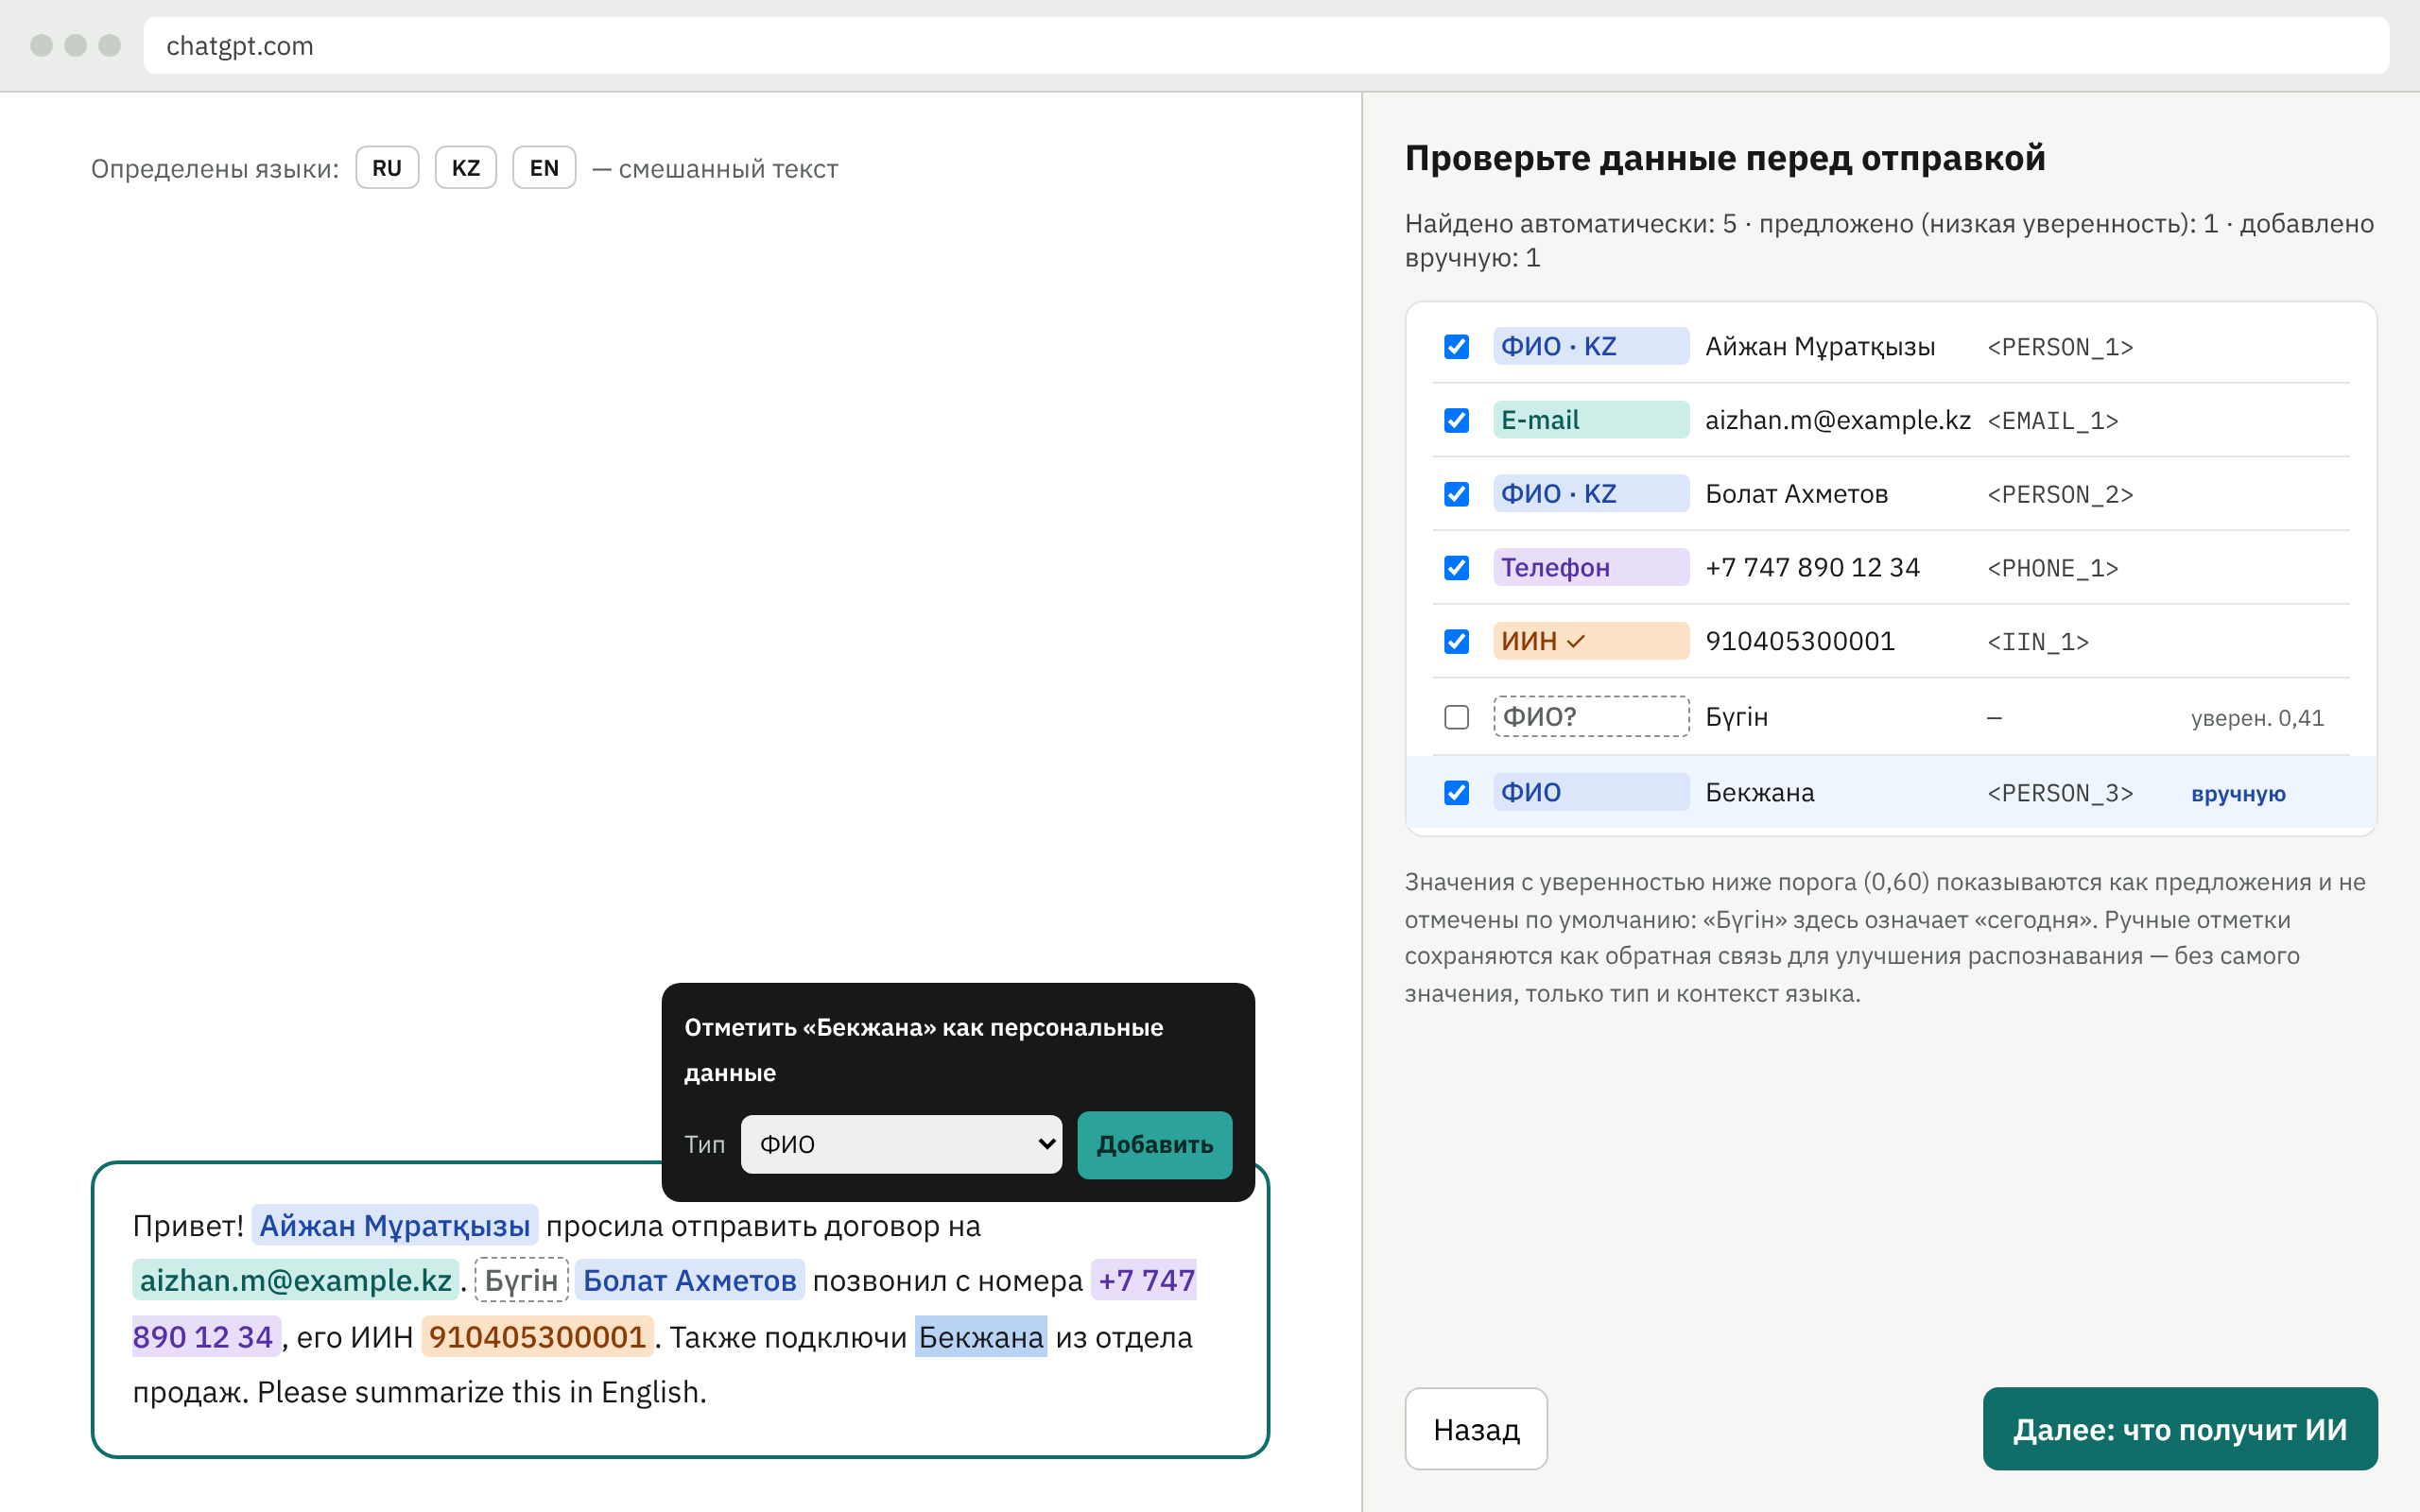
\includegraphics[width=\linewidth]{07-U7-Mixed.png}
\caption{U7. Mixed Kazakh--Russian--English text: a low-confidence suggestion is not marked by default, and a missed name is added manually}\label{fig:u7}
\end{figure}

\begin{figure}[H]
\centering
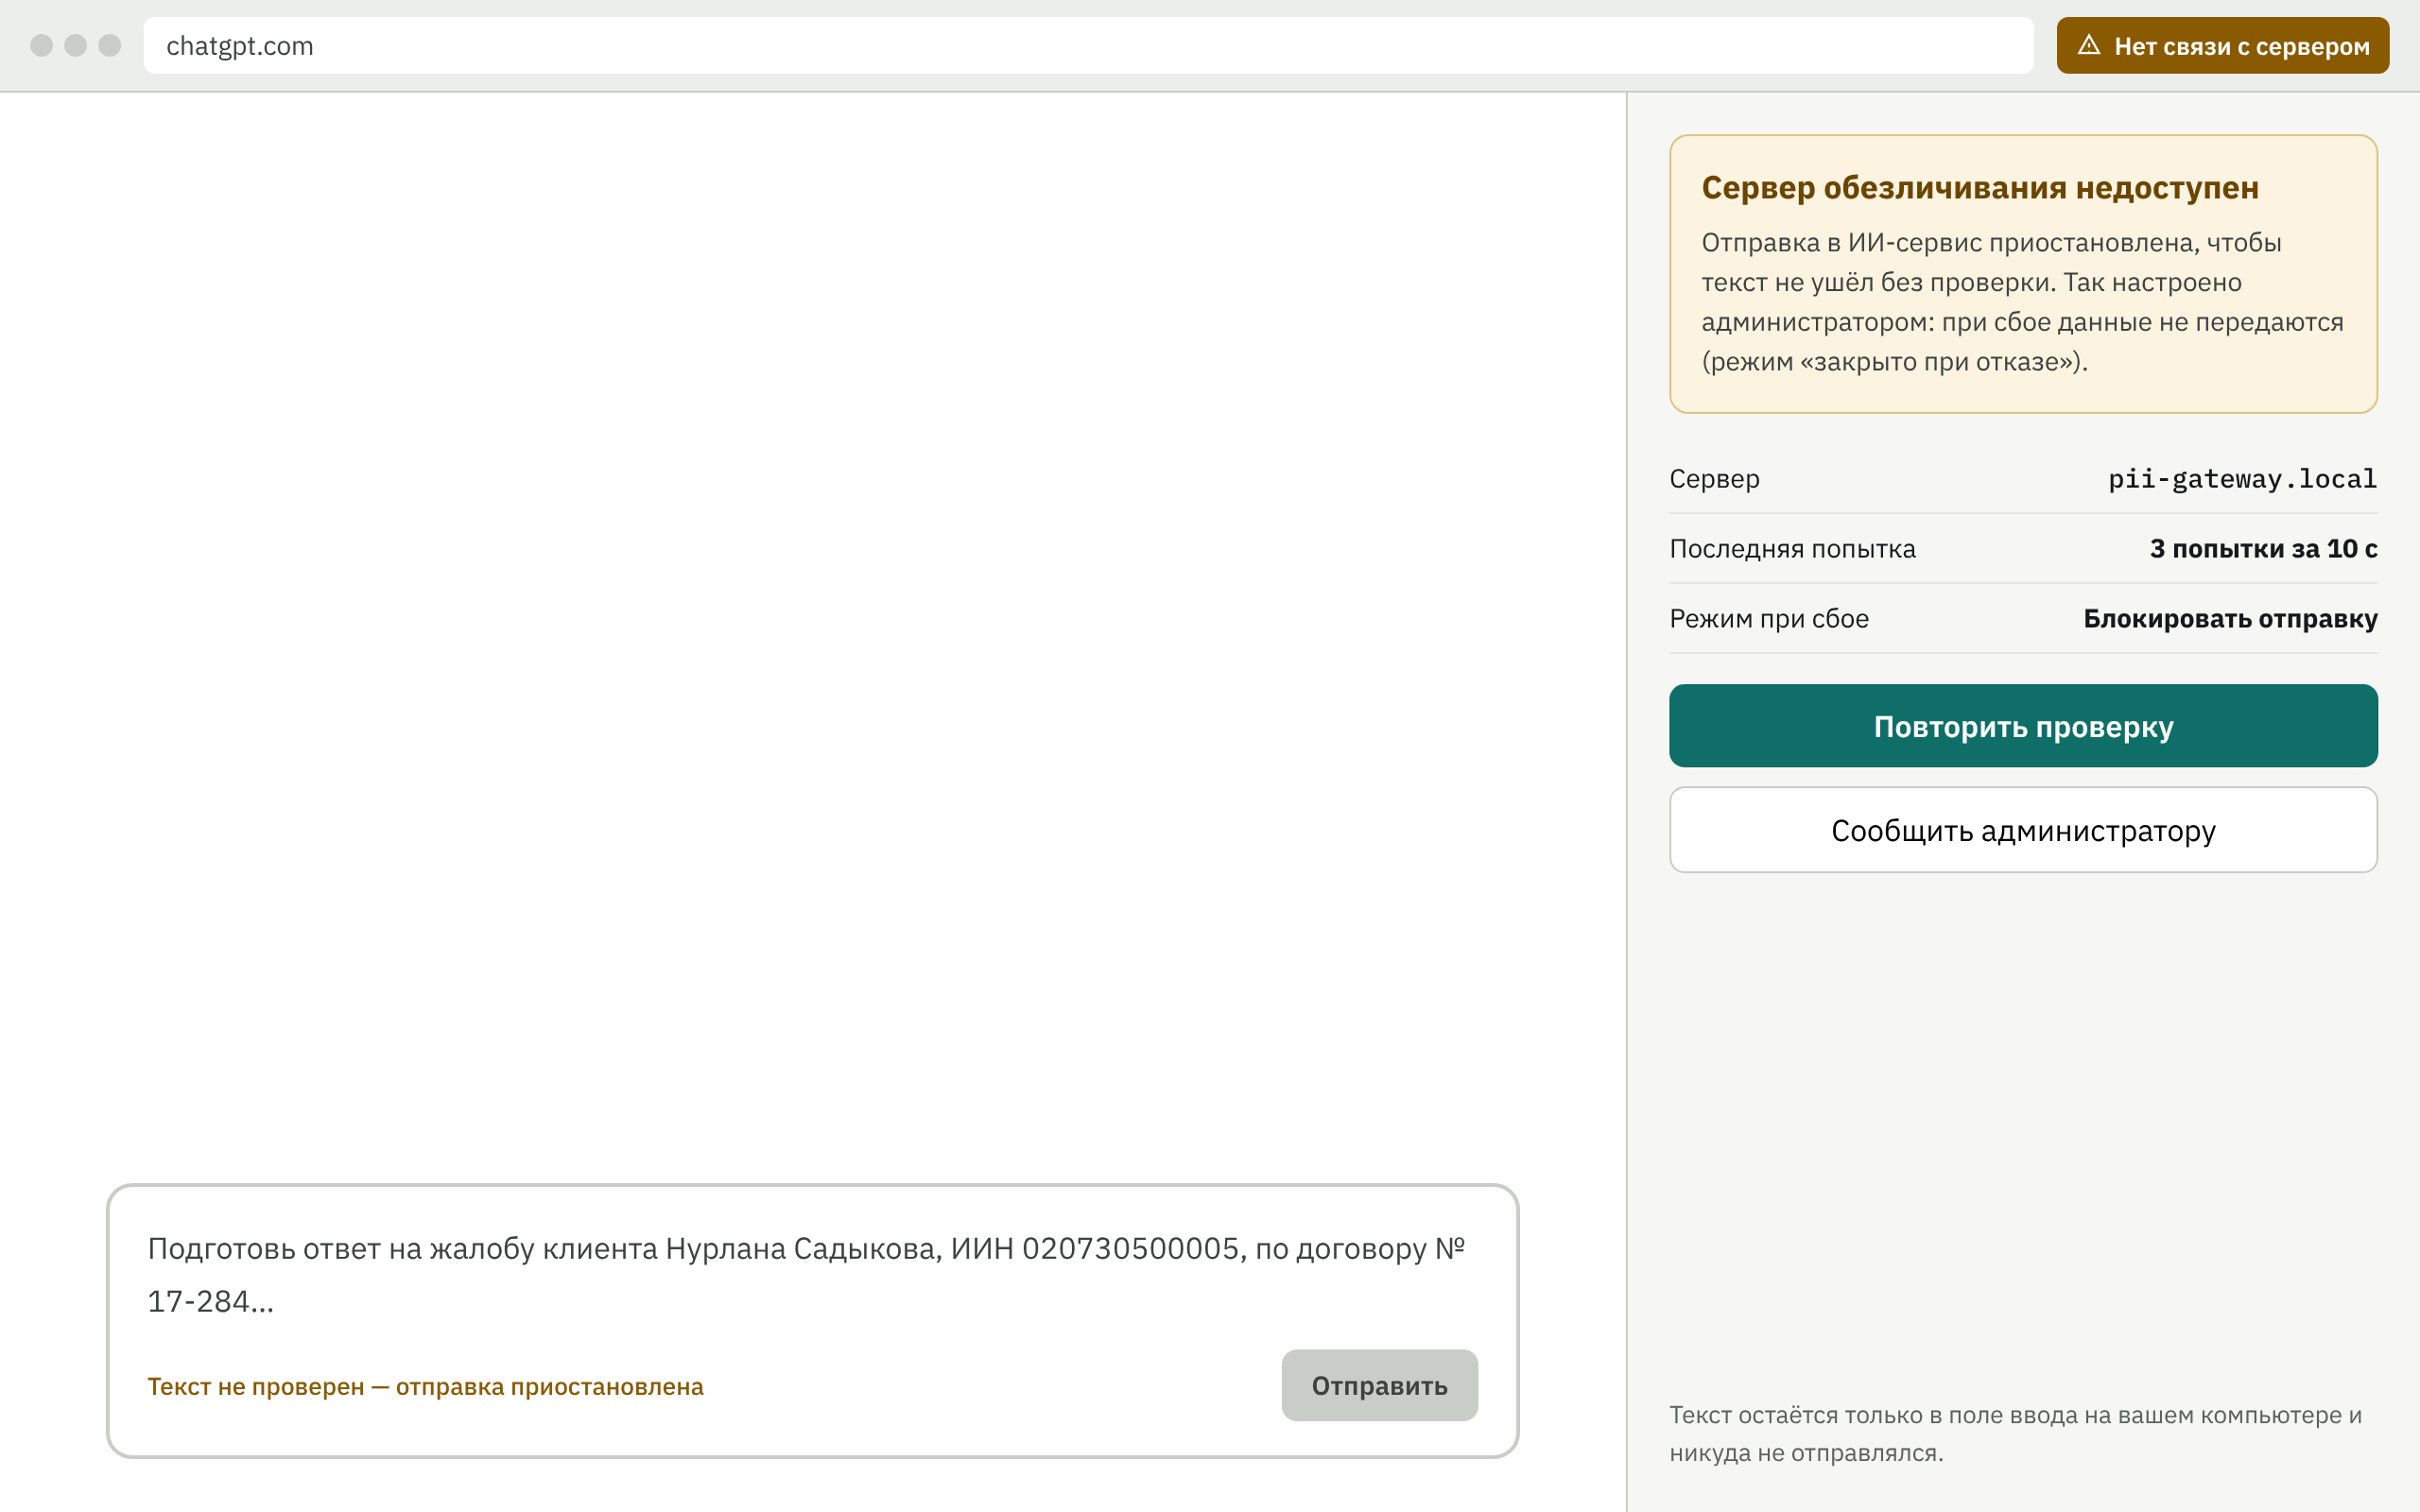
\includegraphics[width=\linewidth]{08-U8-Unavailable.png}
\caption{U8. Anonymization server unavailable: sending is suspended so that the text does not leave unchecked (fail-closed)}\label{fig:u8}
\end{figure}

\section{Extension Window}

\begin{figure}[H]
\centering
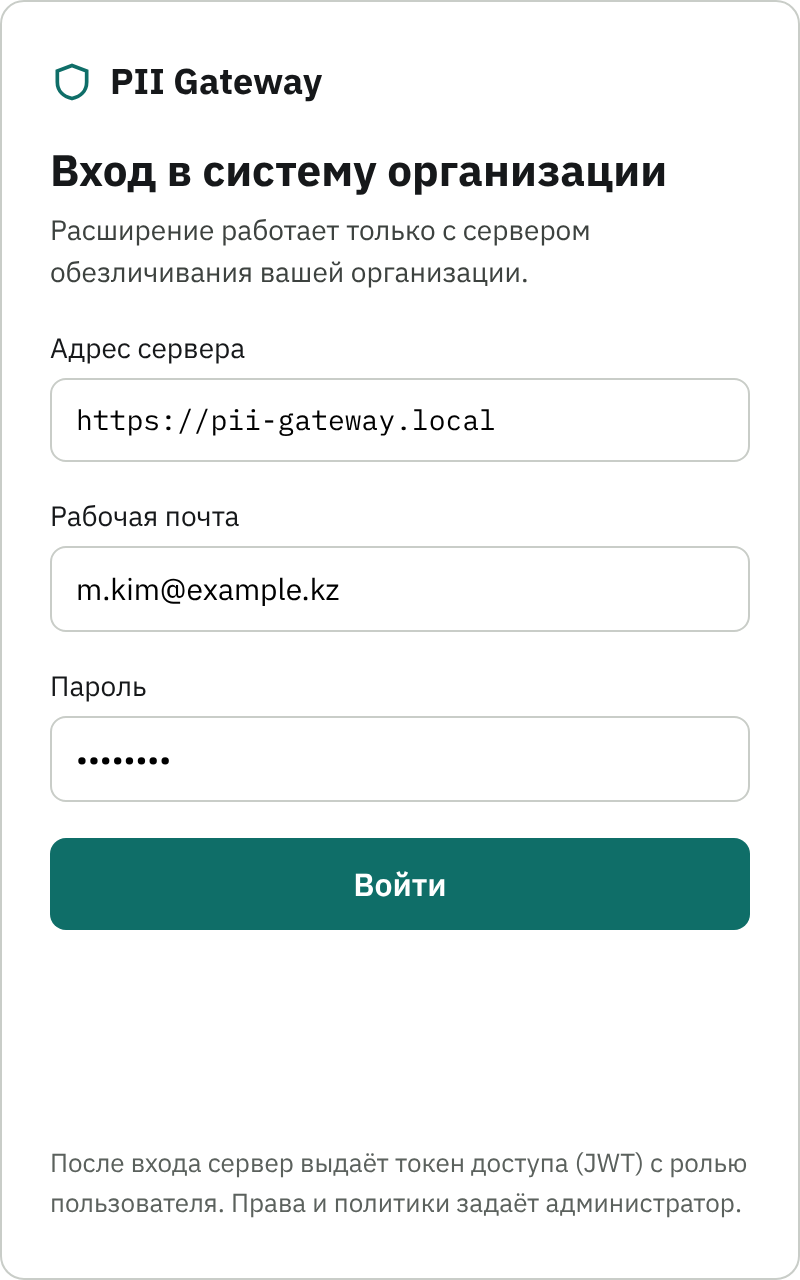
\includegraphics[width=0.36\linewidth]{10-X2-Login.png}\hspace{1cm}
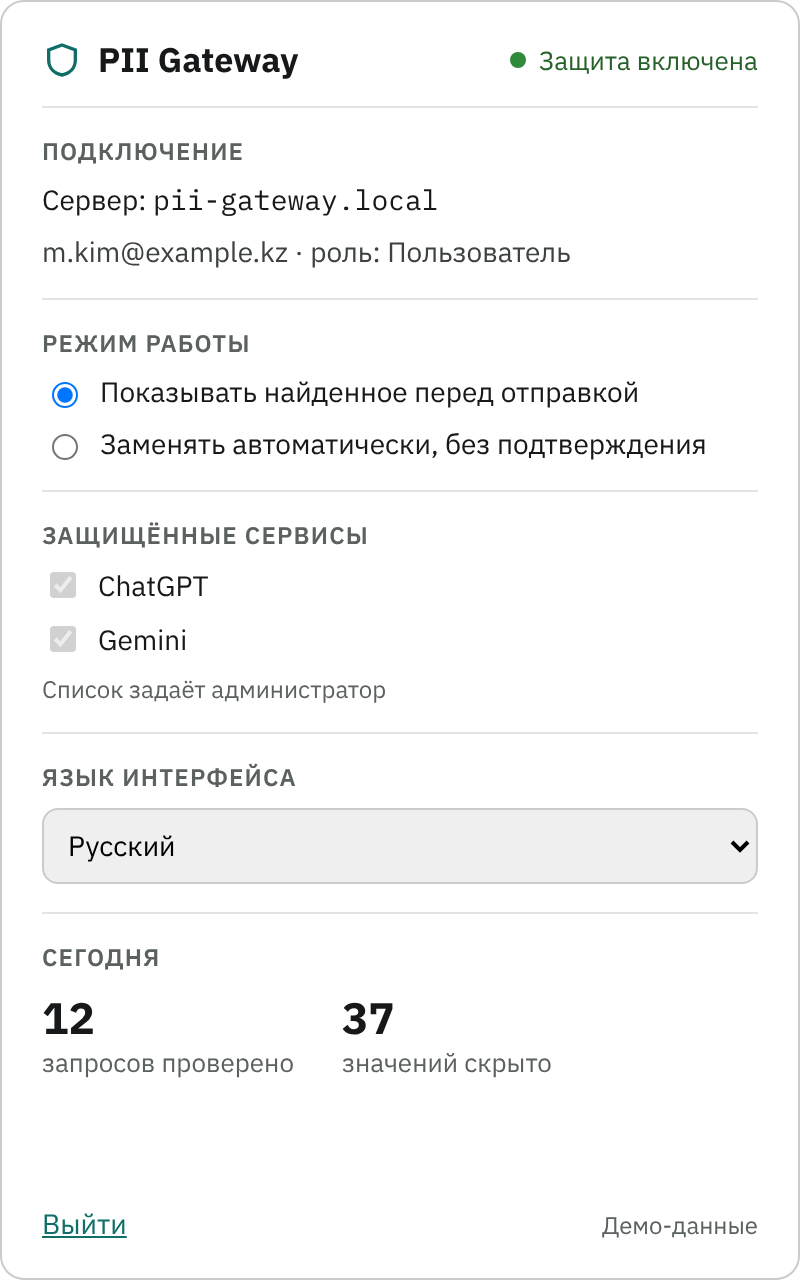
\includegraphics[width=0.36\linewidth]{09-X1-Popup.png}
\caption{X2 (left): sign-in with an organization account; X1 (right): protection status, mode, protected services and interface language}\label{fig:x}
\end{figure}

\section{Administration Panel}

The administration panel is used by the information security service (use cases UC-5 and UC-6). Access is limited to the roles ``Administrator'' and ``Auditor''.

\begin{figure}[H]
\centering
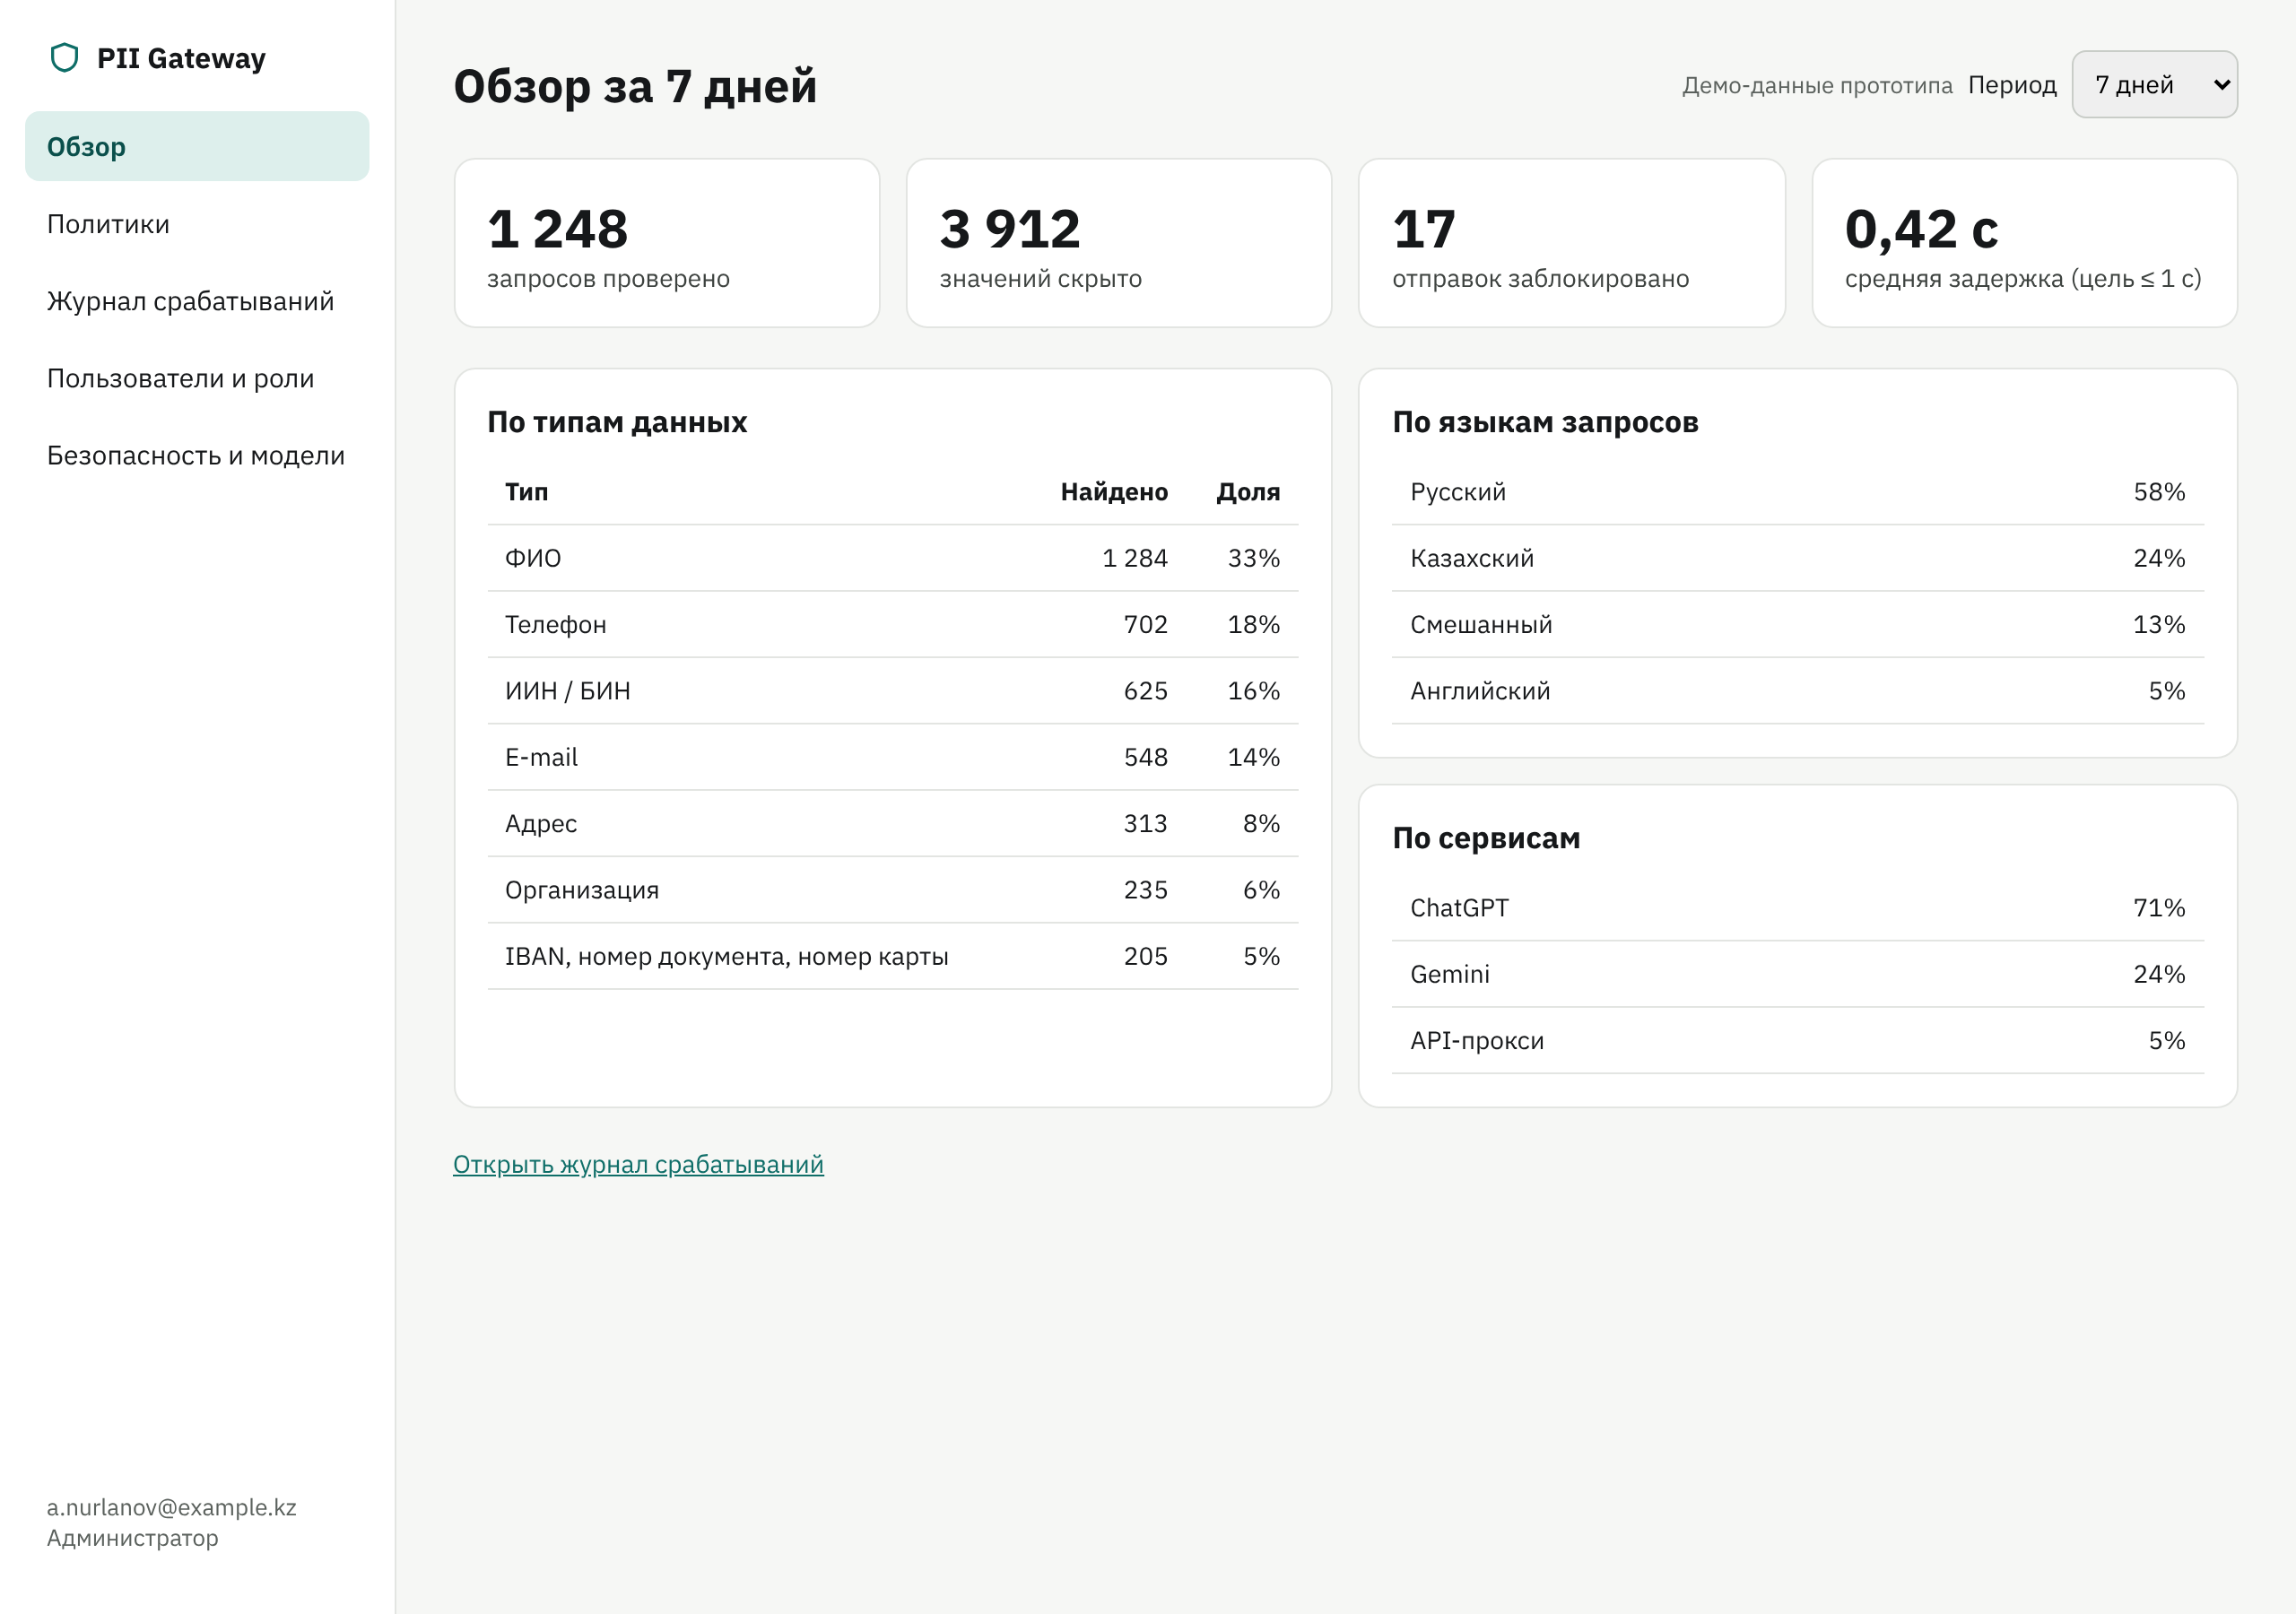
\includegraphics[width=\linewidth]{12-A2-Dashboard.png}
\caption{A2. Statistics: number of checks, hidden values, blocked requests, distribution by data type and average latency}\label{fig:a2}
\end{figure}

\begin{figure}[H]
\centering
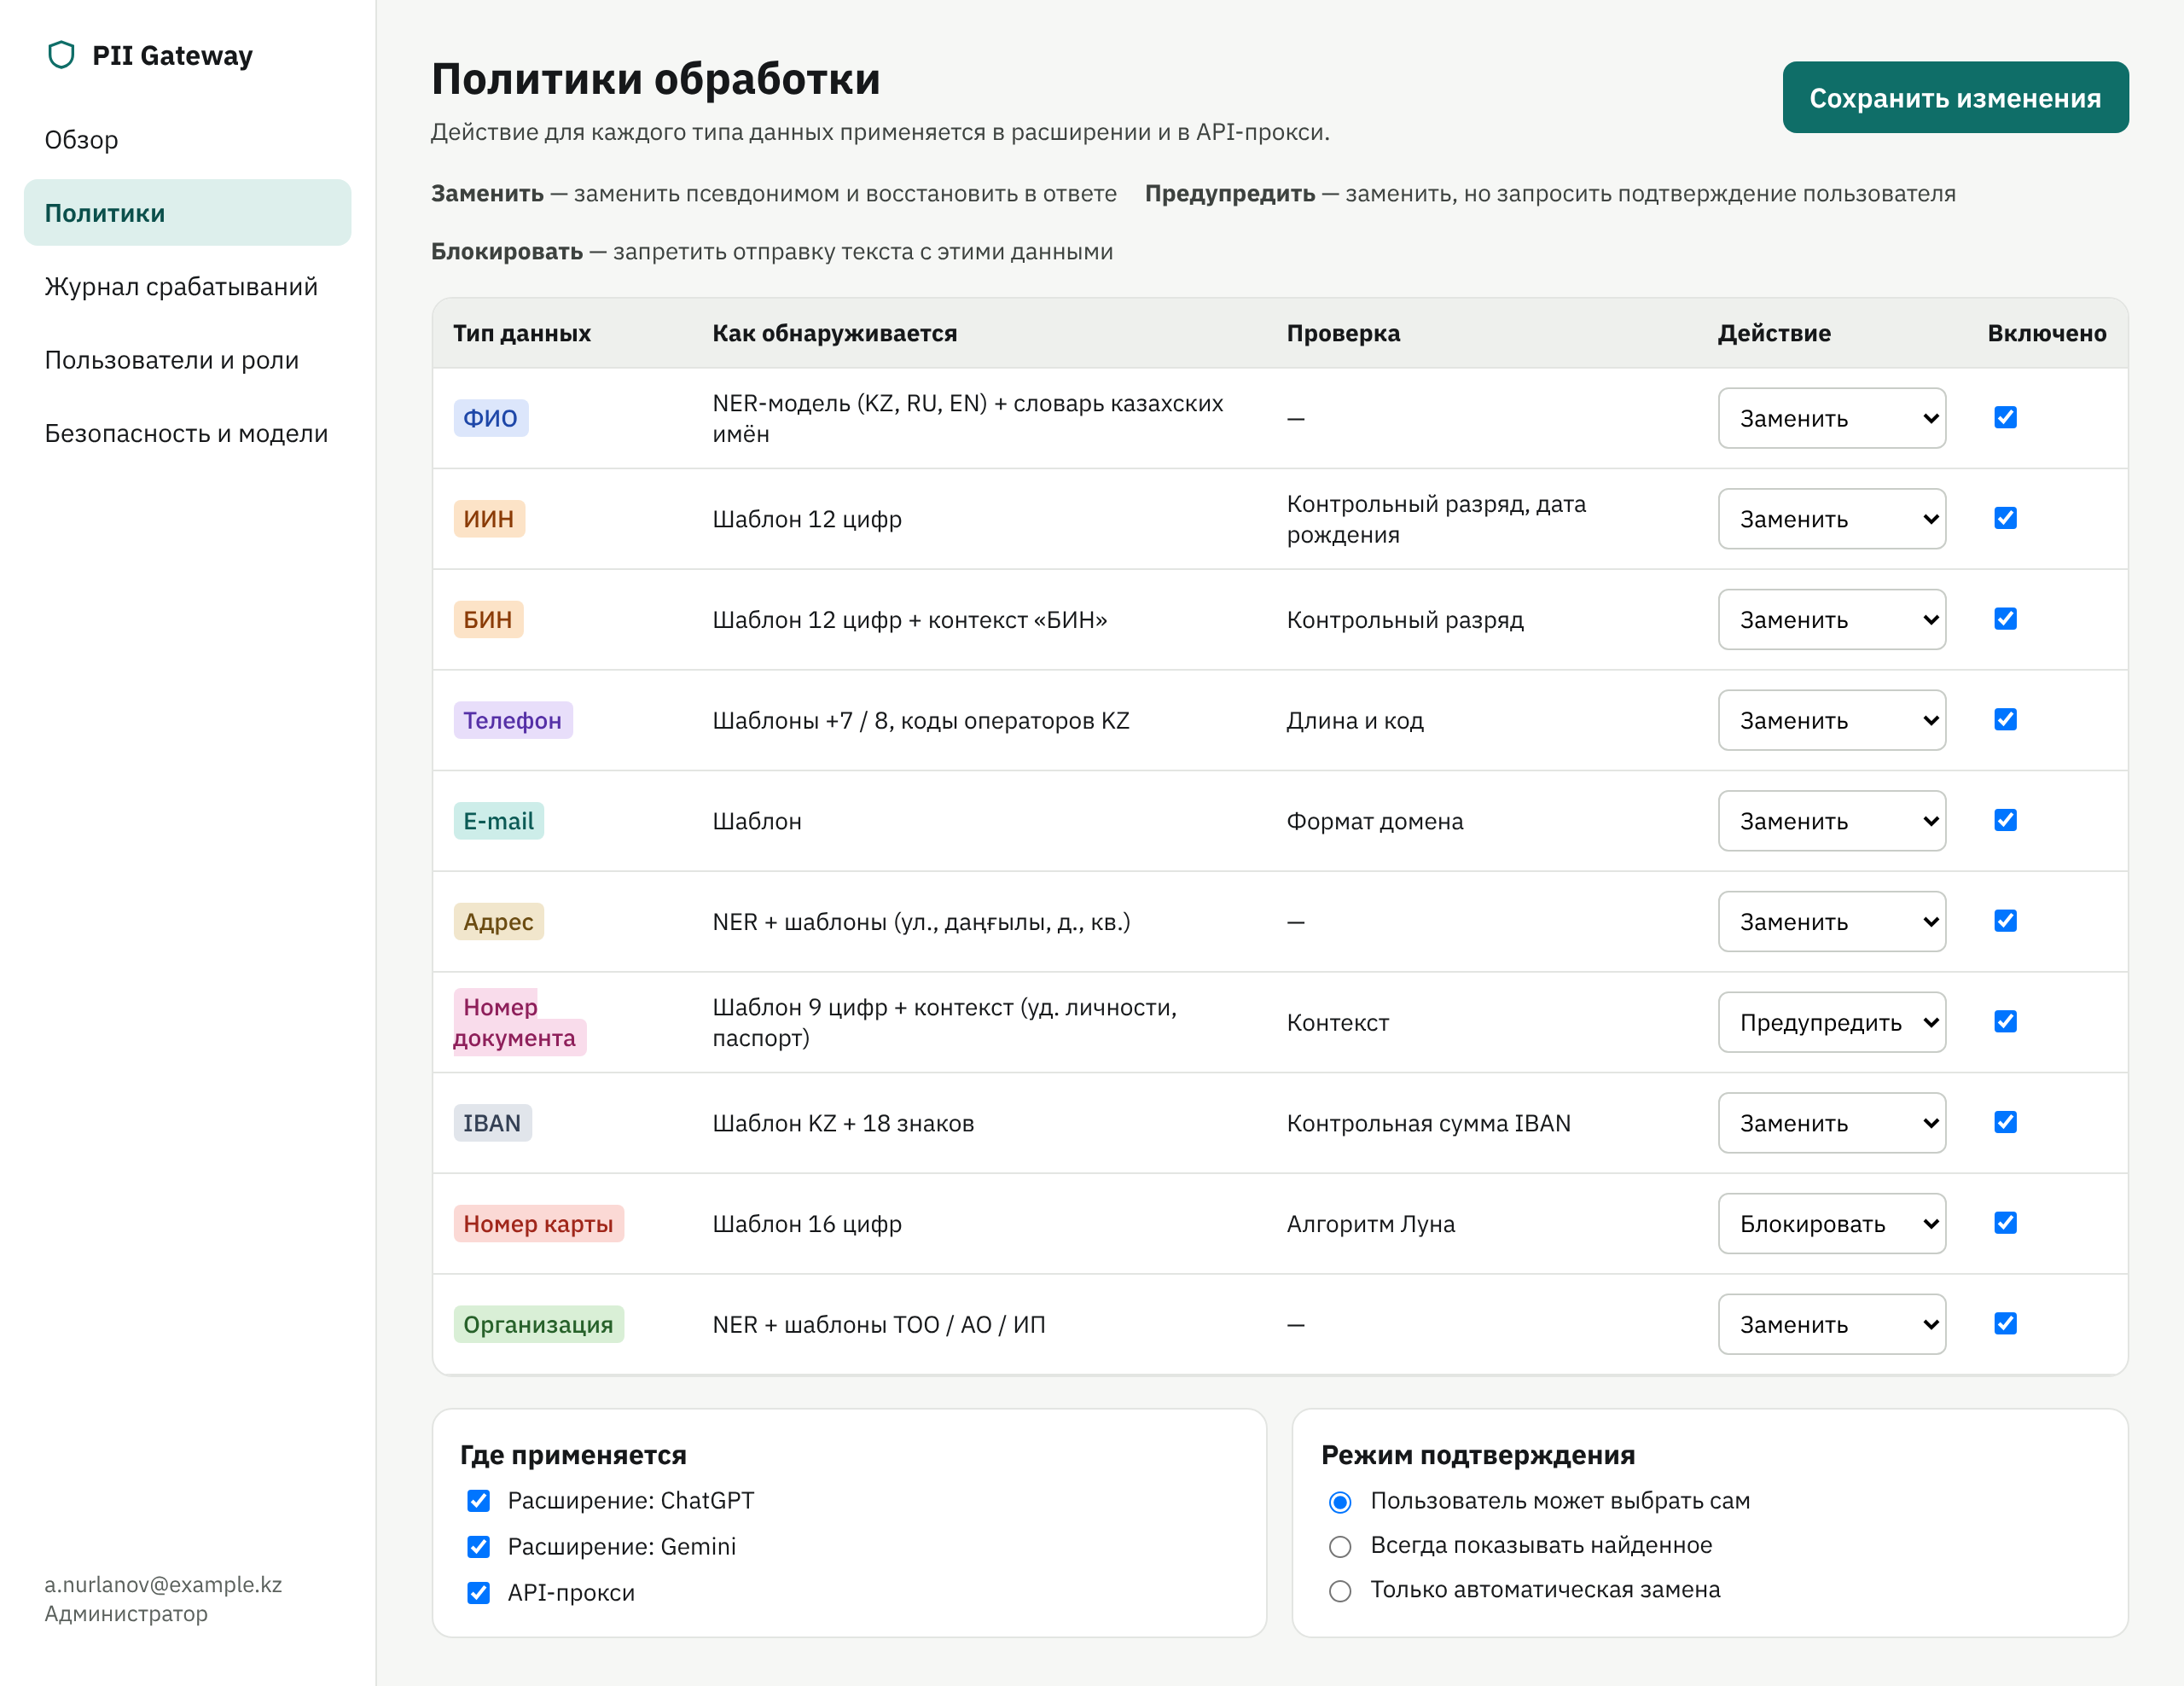
\includegraphics[width=\linewidth]{13-A3-Policies.png}
\caption{A3. Processing policies: detection method, validation and action for each data type}\label{fig:a3}
\end{figure}

\begin{figure}[H]
\centering
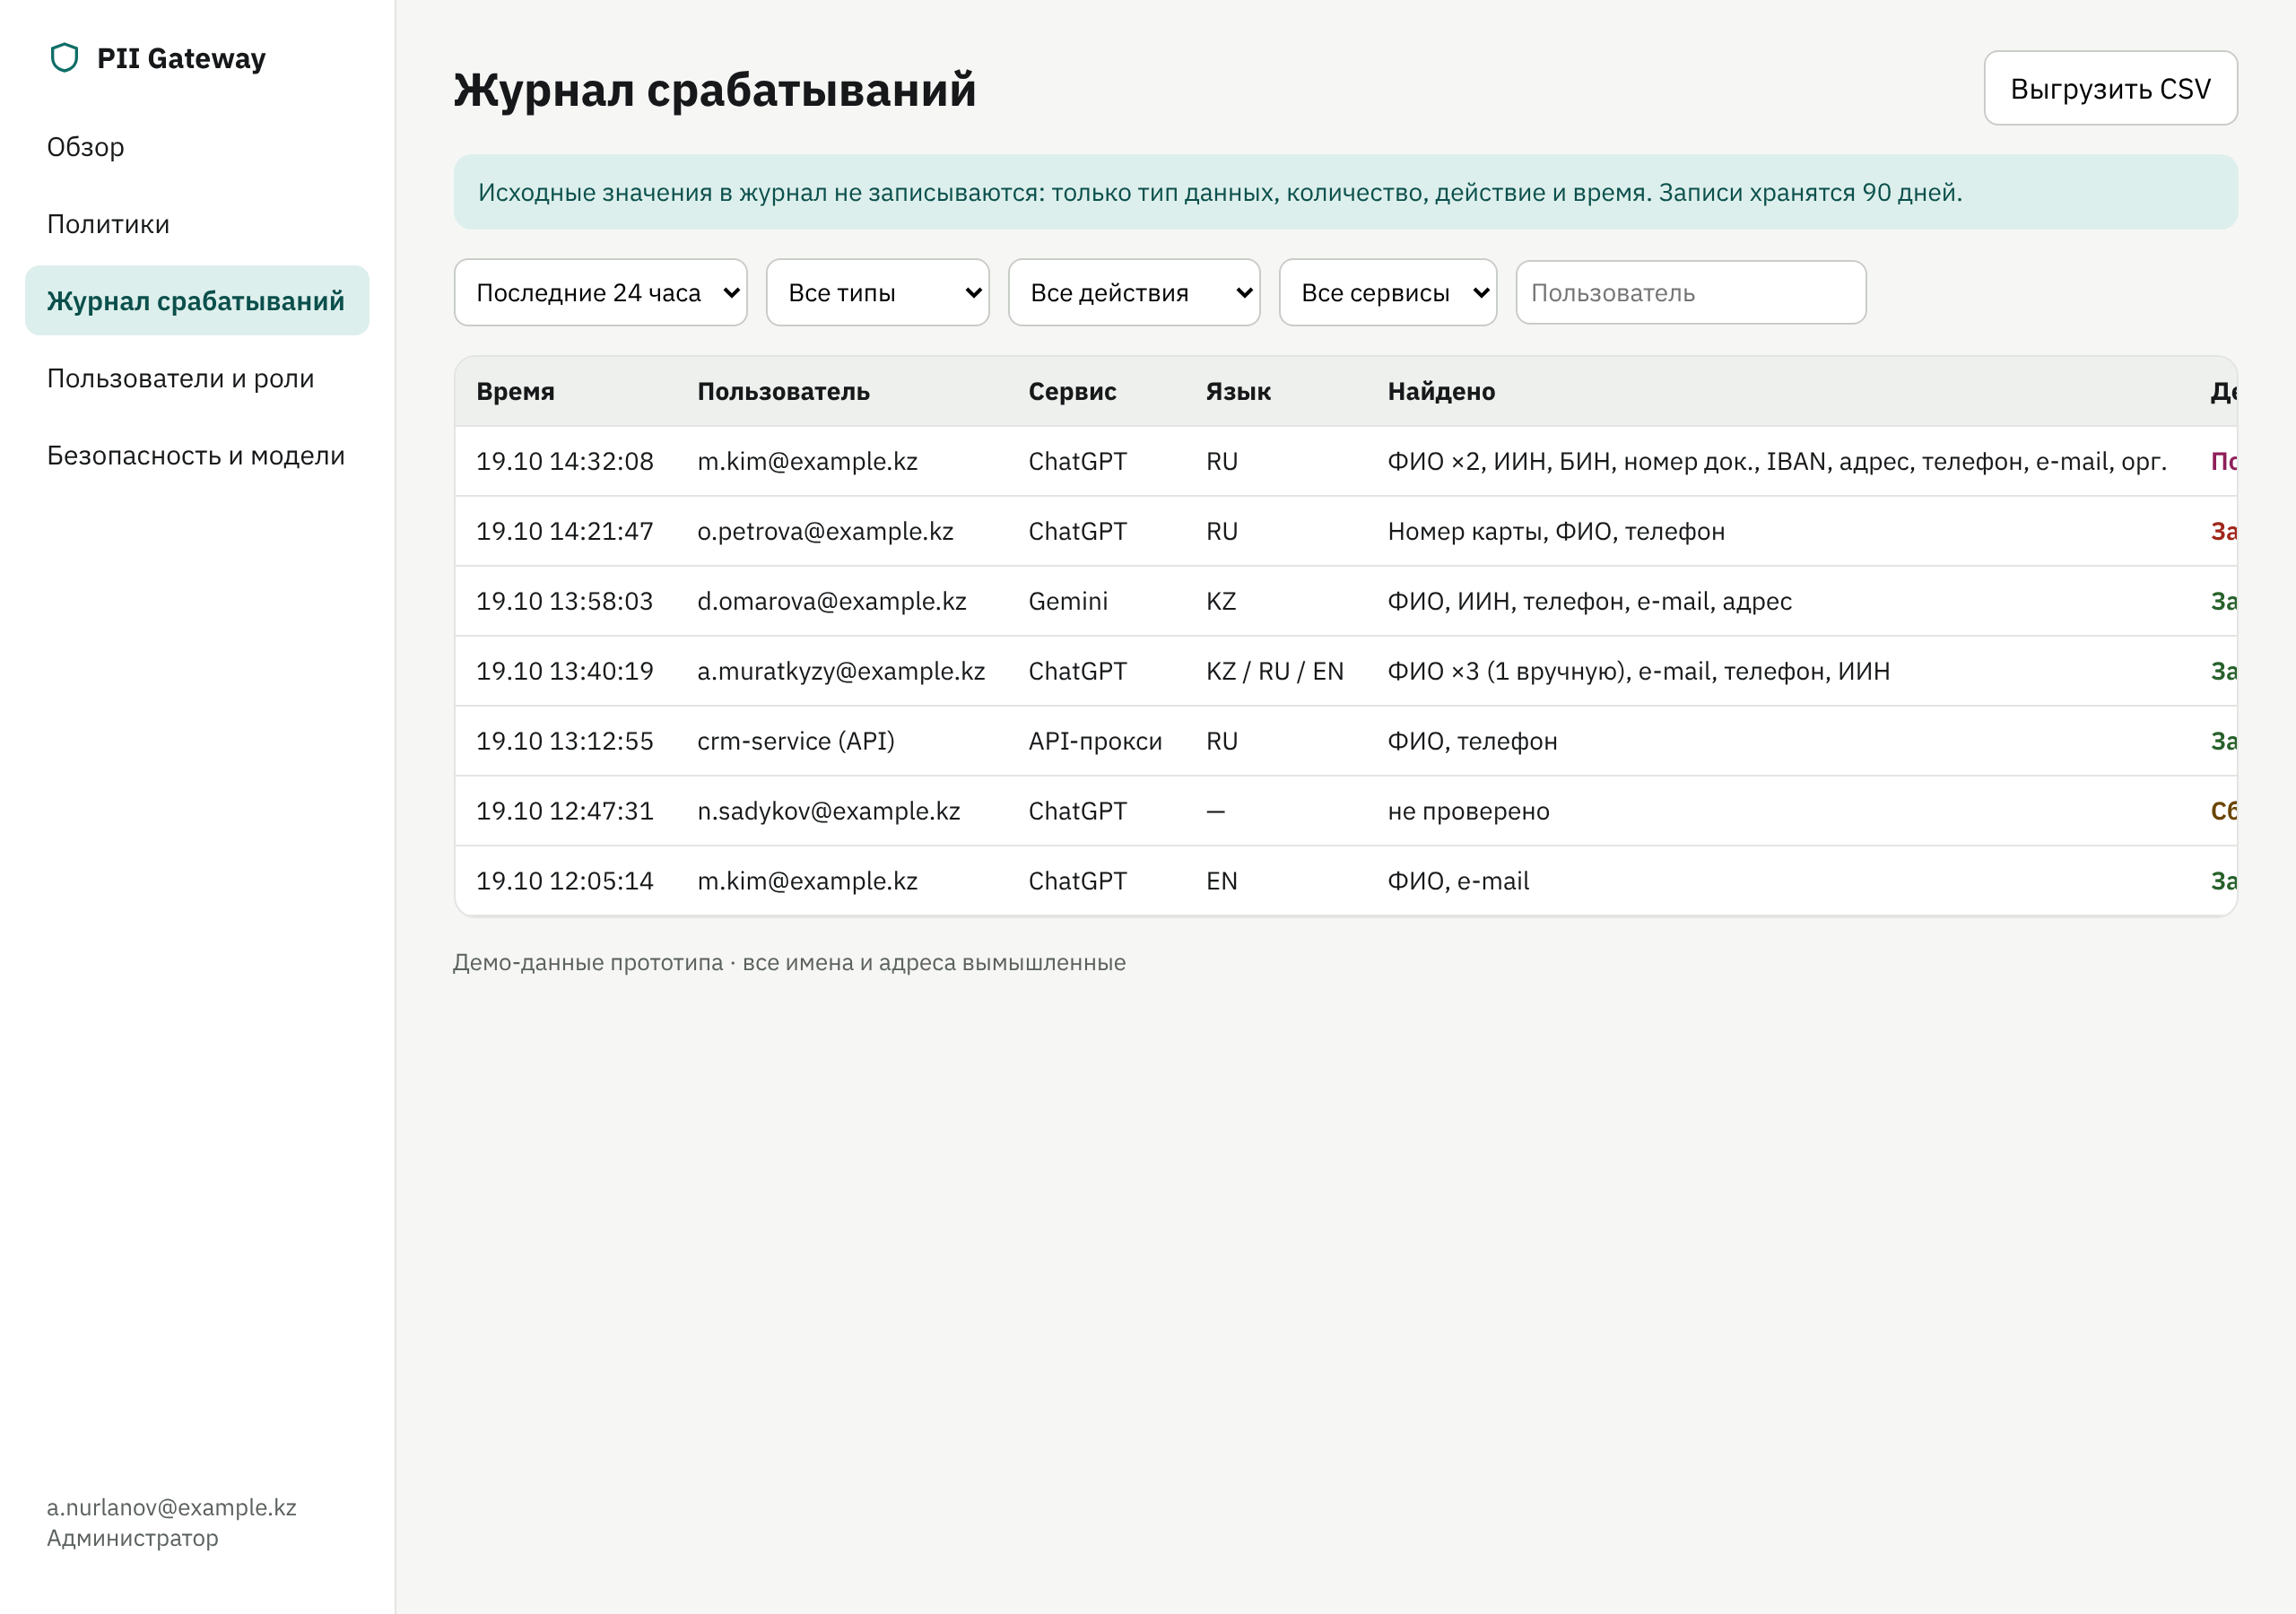
\includegraphics[width=\linewidth]{14-A4-Logs.png}
\caption{A4. Detection log: only the data type, number of values, action and time are recorded, without original values}\label{fig:a4}
\end{figure}

\begin{figure}[H]
\centering
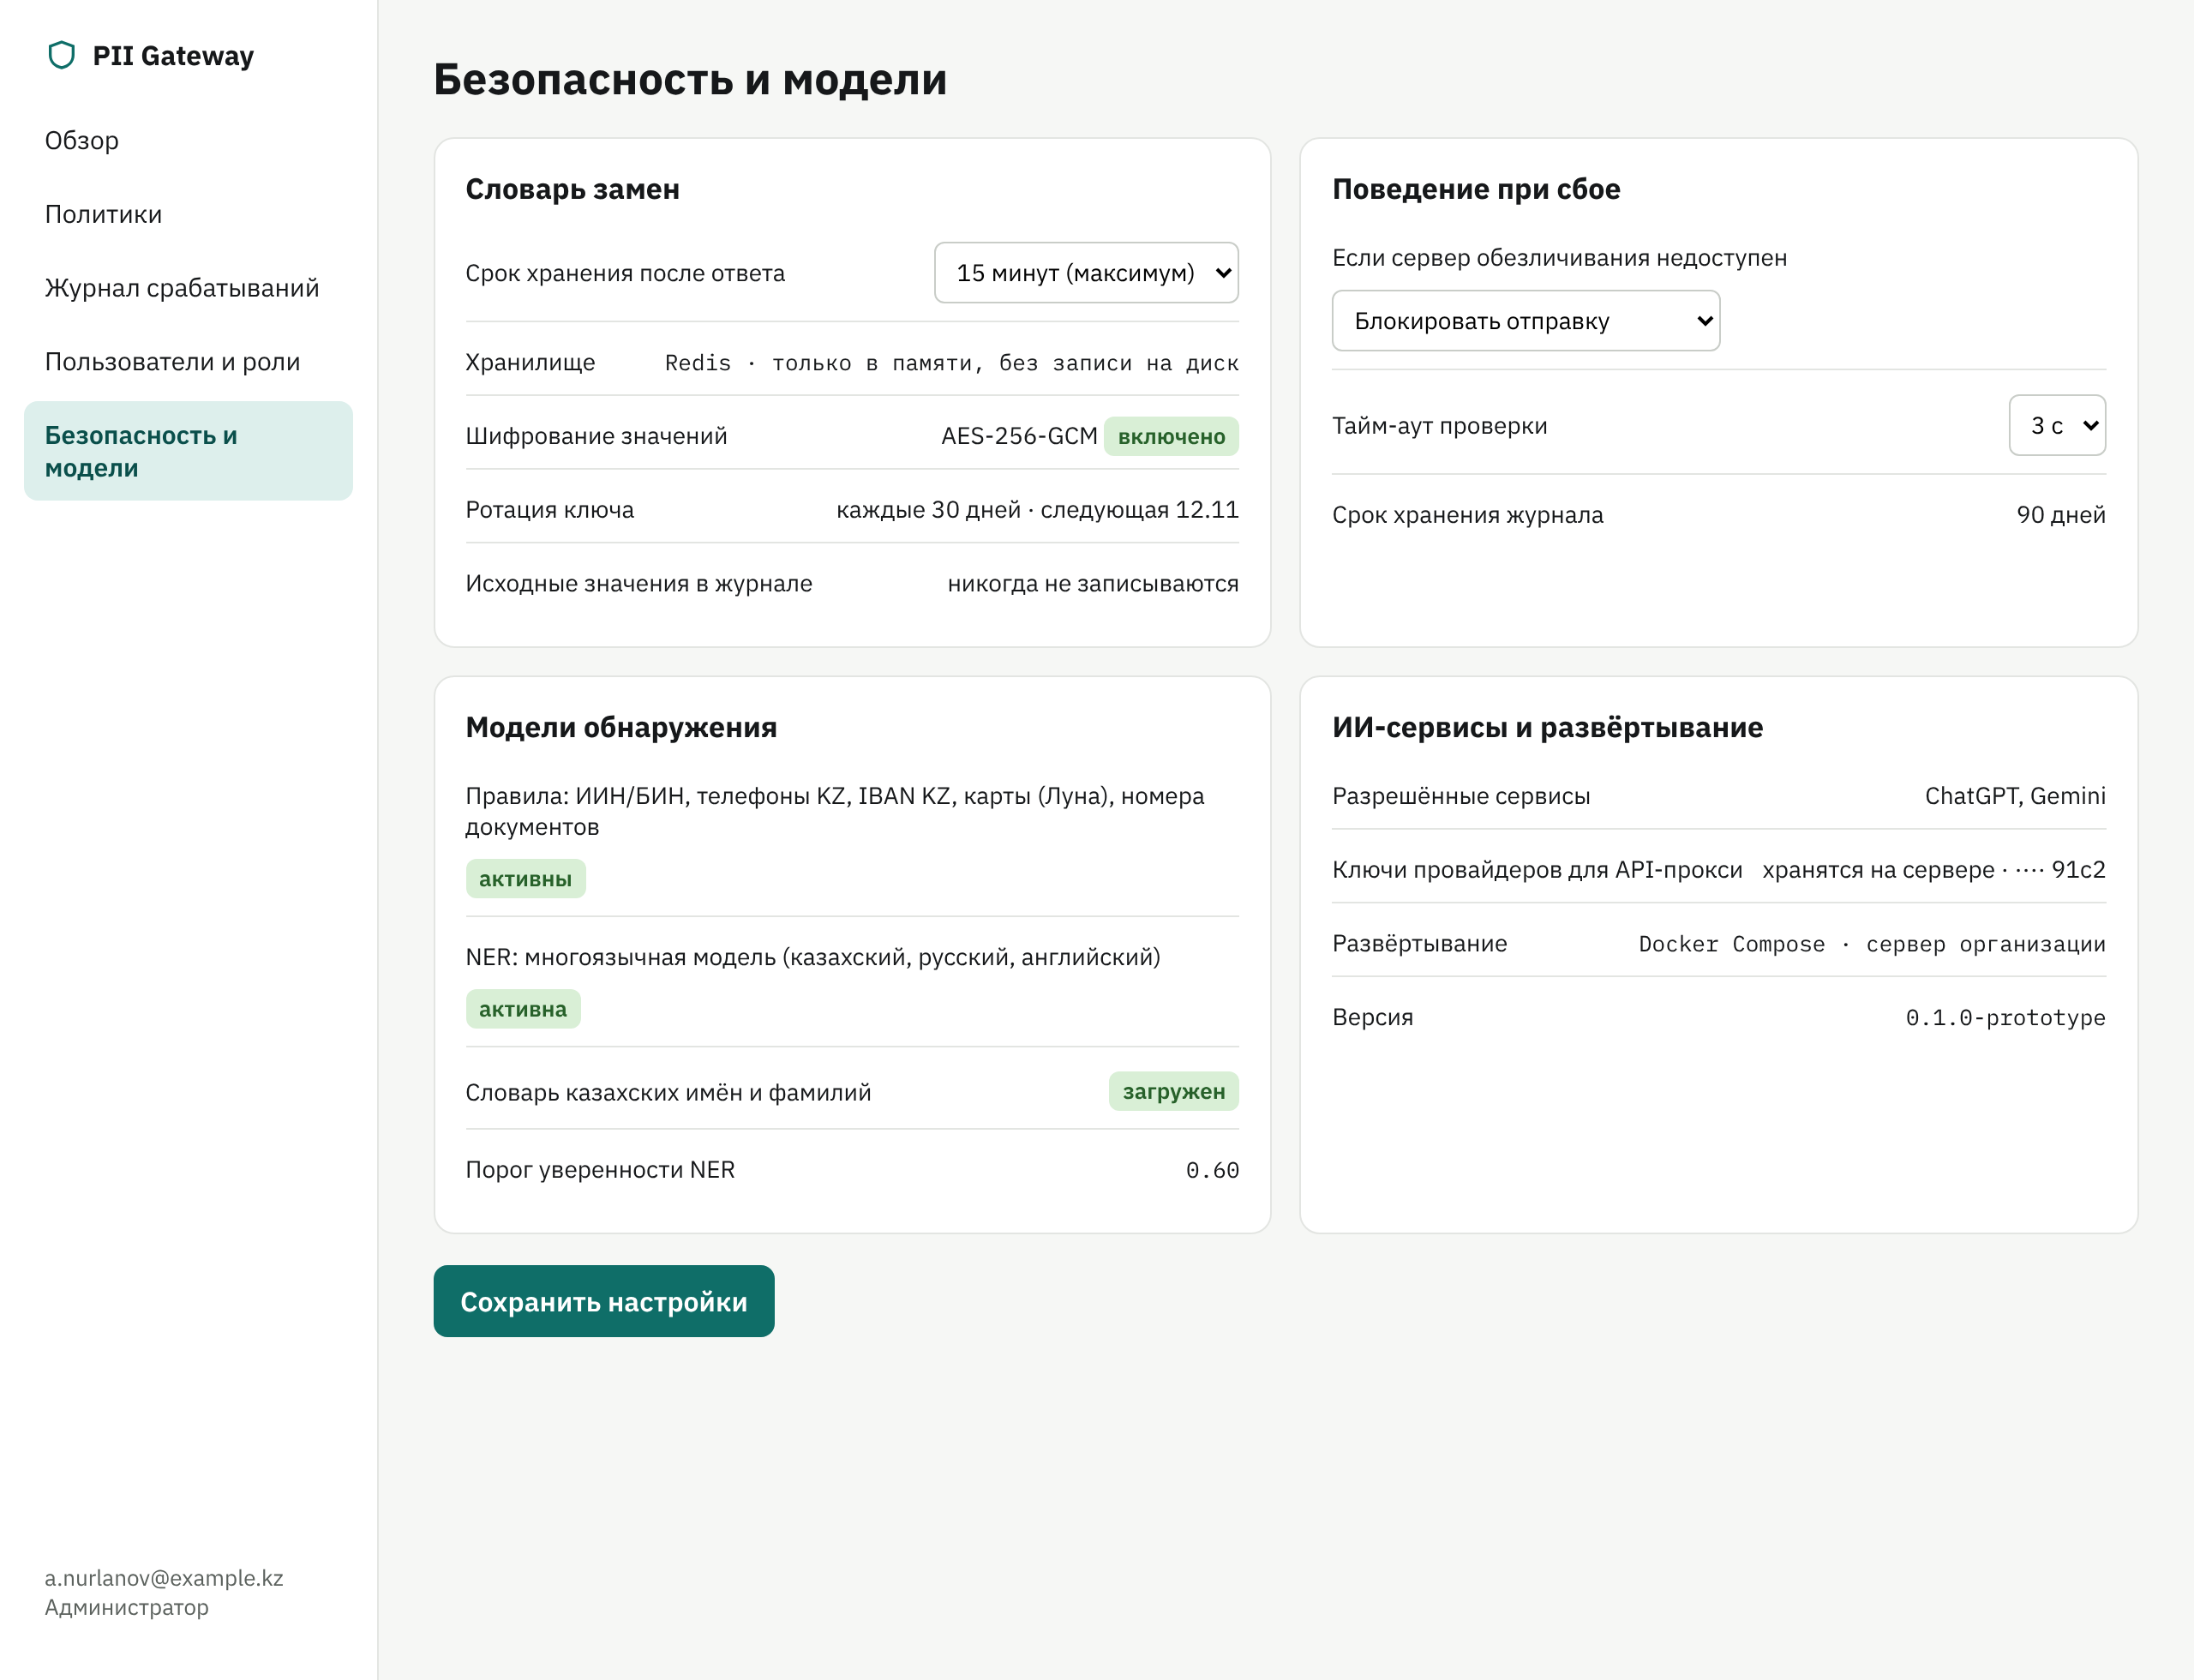
\includegraphics[width=\linewidth]{16-A6-Settings.png}
\caption{A6. Security and models: mapping retention (at most 15 minutes), encryption, behaviour on failure, log retention and status of detection models}\label{fig:a6}
\end{figure}

Screens A1 (sign-in) and A5 (users and roles) are included in the repository and listed in Table~\ref{tab:screens}.

\section{Programming Interface}

Screen P1 (Figure~\ref{fig:p1}) shows the requests and responses of the anonymization endpoint and of the proxy compatible with the OpenAI chat interface, which are used by service accounts (UC-4).

\begin{figure}[H]
\centering
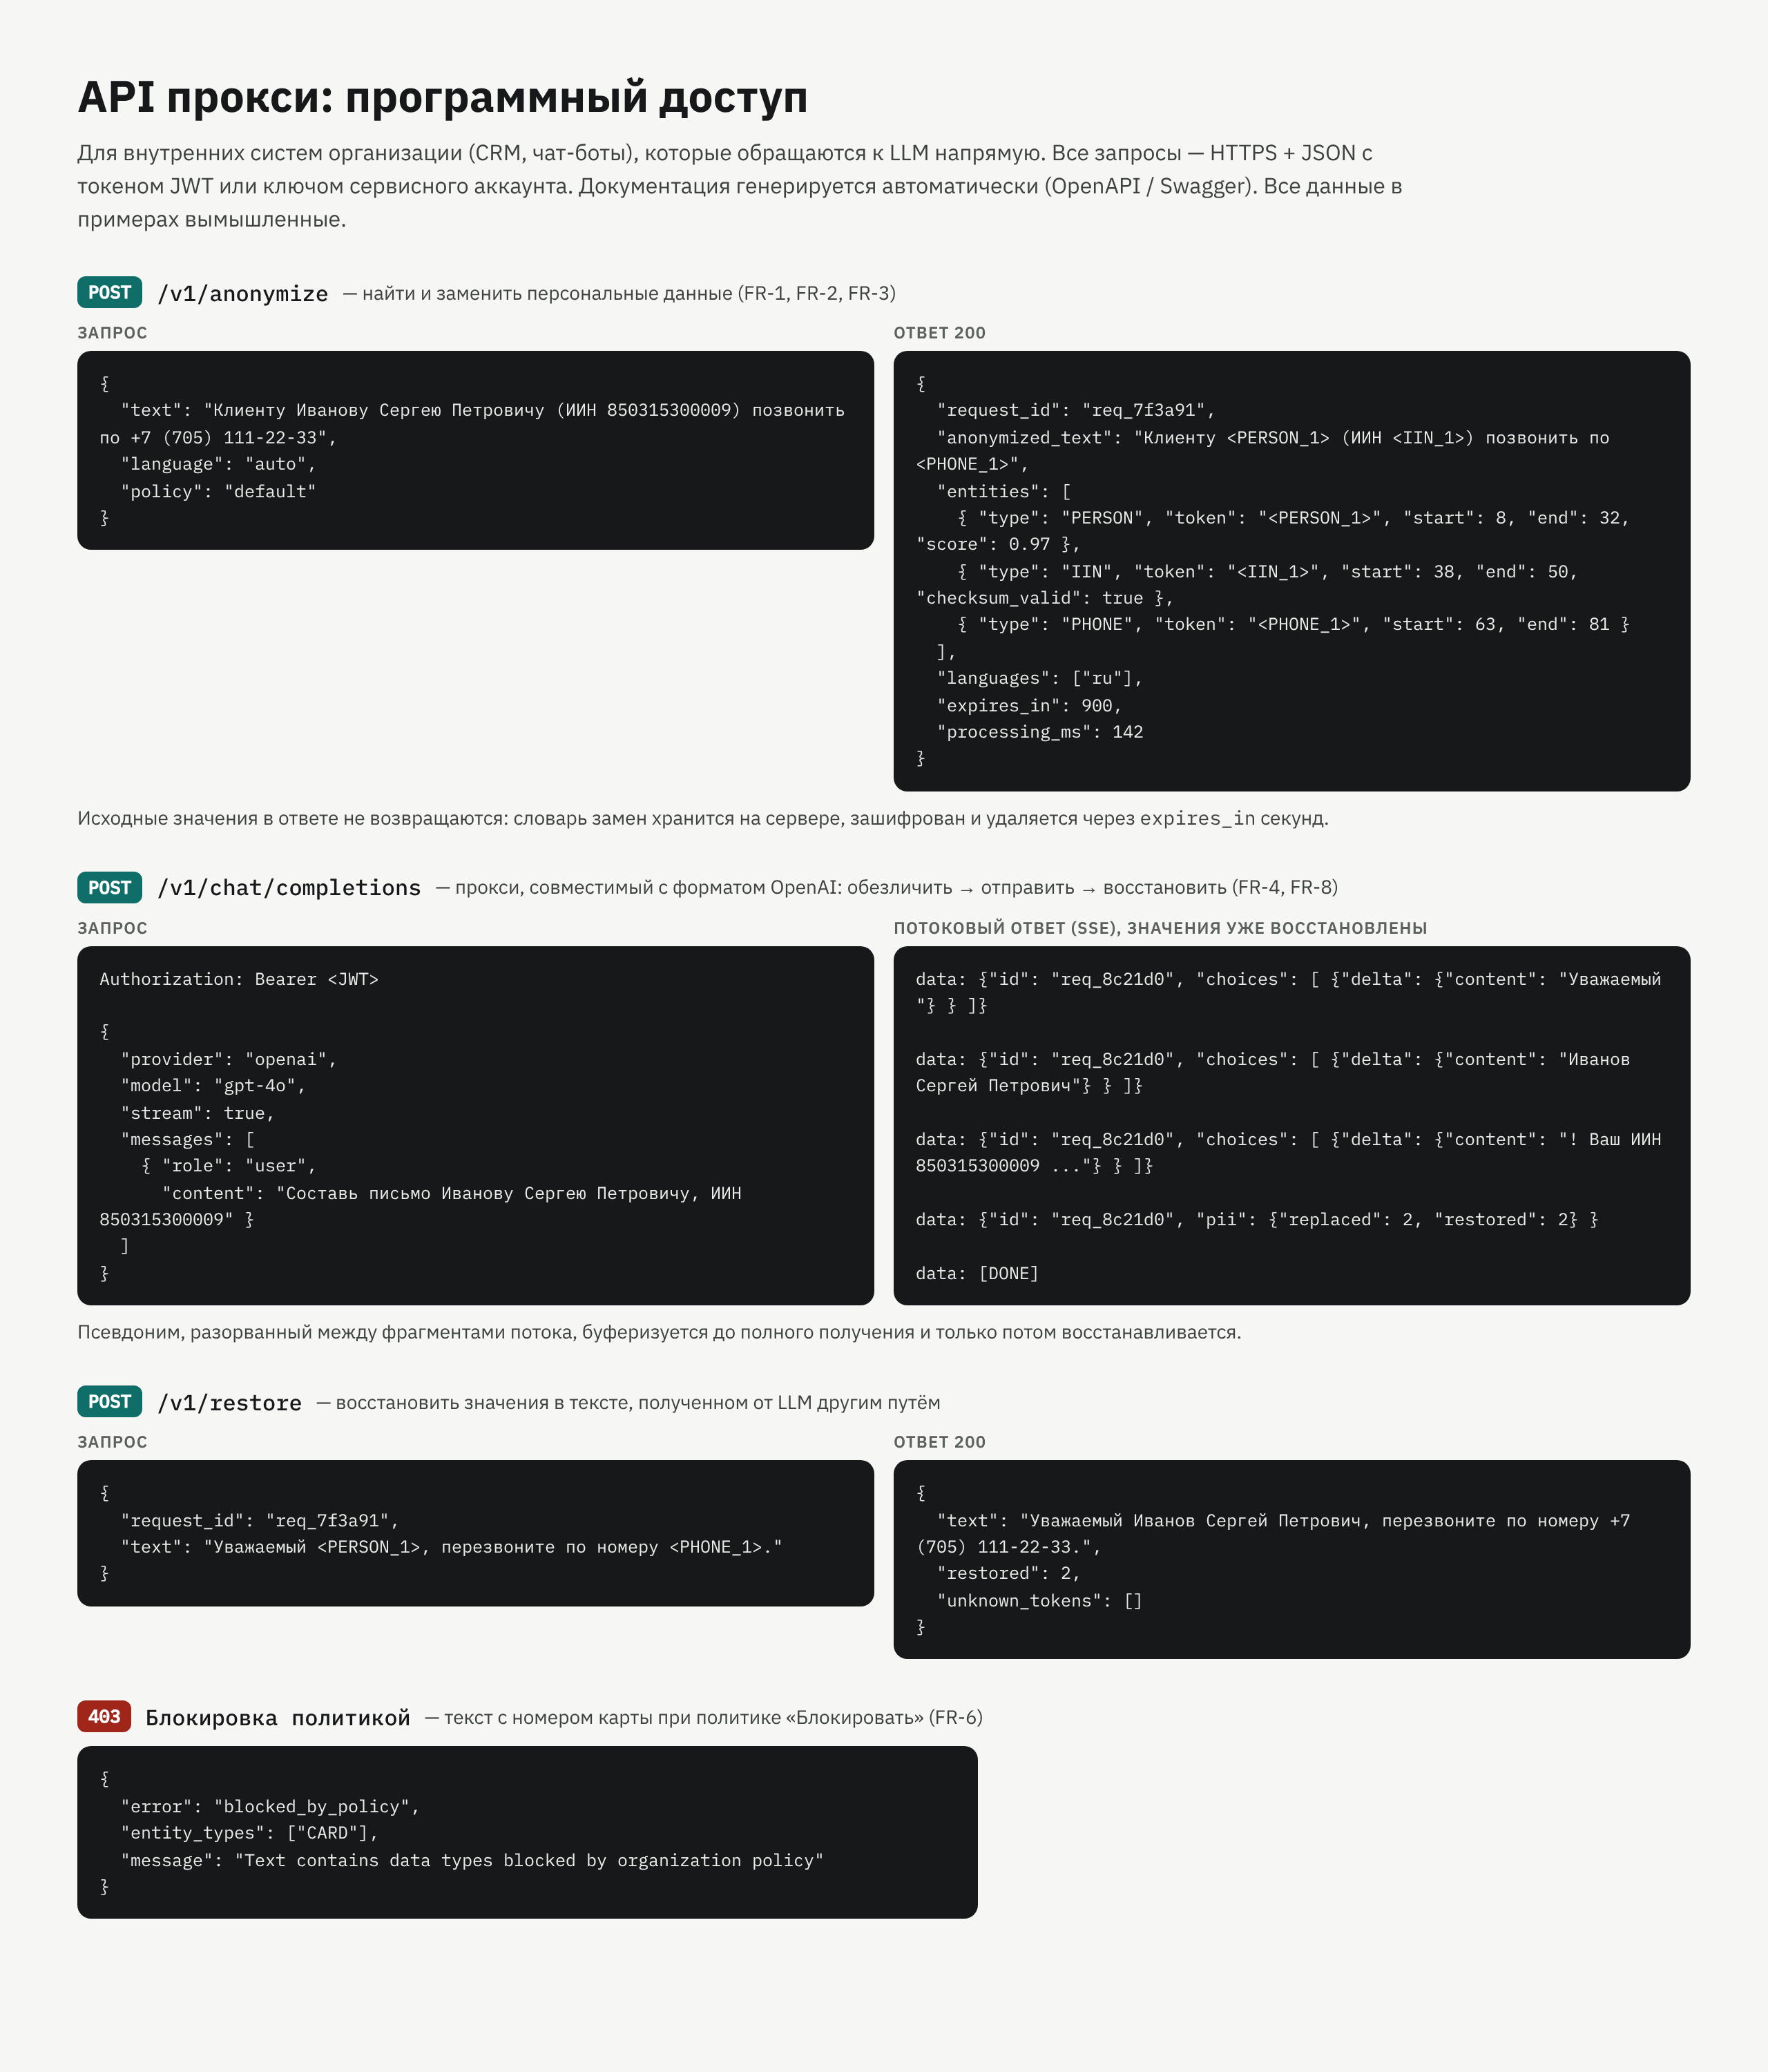
\includegraphics[height=0.72\textheight]{17-P1-API.png}
\caption{P1. API examples: anonymization, proxy to the language model with a streamed response, and restoration}\label{fig:p1}
\end{figure}

\section{Screens and Requirements}

Table~\ref{tab:screens} links each screen to the requirements it demonstrates. Every functional requirement FR-1--FR-8 and the user-facing non-functional requirements are covered by at least one screen.

{\small
\renewcommand{\arraystretch}{1.2}
\begin{xltabular}{\linewidth}{P{1.4cm}P{4.0cm}LP{2.8cm}}
\caption{Screens and requirements}\label{tab:screens}\\
\toprule
\thead \textbf{Screen} & \textbf{Name} & \textbf{What is shown} & \textbf{Requirements} \\ \midrule
\endfirsthead
\multicolumn{4}{l}{\small\textit{Table \ref{tab:screens} (continued)}}\\
\toprule
\thead \textbf{Screen} & \textbf{Name} & \textbf{What is shown} & \textbf{Requirements} \\ \midrule
\endhead
U1 & Text input & Highlighting of all data types, validated IIN and BIN & FR-1, FR-2, FR-5.1 \\ \rl
U2 & Review of detected data & Review list, unmarking, type change, manual marking, ``warn'' policy & FR-3.2, FR-5.2, FR-5.3, FR-6.1 \\ \rl
U3 & Preview & Text received by the AI service, processing time & FR-3.1, FR-5.4, NFR-1 \\ \rl
U4 & Restored response & Streamed response with restored values, view ``as the AI saw it'' & FR-4.1, FR-4.2, FR-4.4 \\ \rl
U5 & Blocking & Card number blocked by policy, reason shown & FR-2.2, FR-6.1, FR-6.2 \\ \rl
U6 & Kazakh text, Gemini & Kazakh interface, IIN in Kazakh text, second AI service & FR-1.1, FR-5.1, FR-5.7 \\ \rl
U7 & Mixed text & Detected languages, low-confidence suggestion, manual marking & FR-1.3, FR-5.2, FR-5.3 \\ \rl
U8 & Server unavailable & Sending suspended & NFR-4 \\ \rl
X1 & Extension window & Status, mode, protected services, interface language & FR-5.5, FR-5.7, FR-6.3 \\ \rl
X2 & Extension sign-in & Organization account, token & FR-5.6, NFR-2 \\ \rl
A1 & Panel sign-in & Access for administrators and auditors only & FR-7.4, NFR-2 \\ \rl
A2 & Statistics & Checks, hidden values, blocks, latency & FR-7.3, NFR-1 \\ \rl
A3 & Policies & Action per data type, where policies apply & FR-6.1, FR-6.3 \\ \rl
A4 & Log & Filters, CSV export, no original values & FR-7.1, FR-7.2 \\ \rl
A5 & Users and roles & Administrator, auditor, user, service account & FR-7.4 \\ \rl
A6 & Security and models & Retention, encryption, failure behaviour, NER threshold & FR-7.5, NFR-2, NFR-4 \\ \rl
P1 & API & Anonymization endpoint, OpenAI-compatible proxy, restoration & FR-4, FR-8 \\
\bottomrule
\end{xltabular}
}

\section{Usability Testing Plan}

The prototype will be tested with 8--10 participants from the target groups (employees handling personal data and students) before the implementation of the extension user interface. Each participant performs three tasks: sending a request with personal data (U1--U4), handling a blocked request (U5) and adding missed data in a mixed-language text (U7). The following are measured: task completion rate, number of errors, time per task and the System Usability Scale (SUS) score. The target values are a task completion rate of at least 90\% and a SUS score of at least 70 (NFR-5). The results will be used to revise the prototype; the detailed procedure is described in the document \emph{Evaluation Plan}.

\section{Limitations}

The prototype is static: detection results and statistics on the screens are demonstration data and do not reflect the real quality of the system. The web pages of ChatGPT and Gemini are shown as simplified mock-ups, since their actual interfaces change frequently. The administration panel is shown only for desktop screens.

\end{document}
